\chapter{Дискретные бегущие волны в полносвязной системе генераторов Мэки--Гласса}\label{ch:ch2}

В данной главе рассматривается генератор Мэки-Гласса --- электрический генератор, функция напряжения $V(t)$ которого описывается уравнением Мэки-Гласса
%
\begin{equation}
	\dfrac{d V}{dt}=
	- bV+\dfrac{acV(t - \tau) }{1 + (cV(t - \tau))^{\gamma}}.
\end{equation}
%
Здесь $V = V(t) > 0$ --- скалярная функция, $a, b, c, \tau, \gamma$ --- положительные параметры. Параметр $\tau$ --- запаздывание по времени, параметр $\gamma$ определяет форму нелинейности.

Рассмотрим полносвязная цепь из $(N + 1)$ генератора Мэки--Гласса, в которой каждый генератор цепи является как принимающим, так и передающим. Такая цепь описывается системой
\small
\begin{equation}
	\label{eq:system_full_generators}
	\dfrac{d V_{j}}{dt}=- bV_{j} + \dfrac{ac\left(V_{j}(t - \tau) + \sum\limits_{k = 0, k\neq j}^{N}V_{k}(t)\right)}{1 + \left(c\left(V_{j}(t - \tau) + \sum\limits_{k = 0, k\neq j}^{N}V_{k}(t)\right)\right)^{\gamma}}, \quad j=0,1,\ldots,N.
\end{equation}
\normalsize

В данной главе будет показано существование у предельной при $\gamma \to +\infty$ для системы \eqref{eq:system_full_generators}, периодических режимов в виде дискретной бегущей волны --- режимов, для которых компоненты решения отличаются друг от друга сдвигом по времени.

Коротко опишем план главы. В разделе \ref{sec:ch2/sect1} формулируется постановка задачи, описывается механизм построения дискретных бегущих волн. В разделе \ref{sec:ch2/sect2} анализируется вспомогательное уравнение со множеством запаздываний, доказывается существование его периодического решения. В разделе \ref{sec:ch2/sect3} доказывается существование периодического решения системы в виде дискретной бегущей волны. В разделе \ref{sec:ch2/sect4} приводятся результаты численного эксперимента.

\section{Постановка задачи}\label{sec:ch2/sect1}

Сделаем в \eqref{eq:system_full_generators} подстановки
%
\begin{equation}
	\label{eq:mg_norm}
	\beta = b \tau, \ \alpha = ac \tau, \ t = \tau \tilde{t}, V_j(t) = \dfrac{1}{c}u_j\left(\dfrac{t}{\tau}\right) = \dfrac{1}{c}u_j(\tilde{t}).
\end{equation}
%
Получим:
%
\begin{equation*}
	\frac{d}{dt} \left(\dfrac{1}{c}u_j\left(\dfrac{t}{\tau}\right)\right)= -\dfrac{\beta}{\tau c}u_j(\tilde{t}) + \dfrac{\alpha}{\tau c}\dfrac{u_j(\tilde{t} - 1) + \sum\limits_{k = 0, k\neq j}^N u_k(\tilde{t})}{1 + \left(u_j(\tilde{t} - 1) + \sum\limits_{k = 0, k\neq j}^N u_k(\tilde{t})\right)^{\gamma}}
\end{equation*}
%
\begin{equation*}
	\frac{1}{\tau} \dot{u}_j(\tilde{t}) = -\dfrac{\beta}{\tau}u_j(\tilde{t}) + \dfrac{\alpha}{\tau}\dfrac{u_j(\tilde{t} - 1) + \sum\limits_{k = 0, k\neq j}^N u_k(\tilde{t})}{1 + \left(u_j(\tilde{t} - 1) + \sum\limits_{k = 0, k\neq j}^N u_k(\tilde{t})\right)^{\gamma}}
\end{equation*}
%
Для удобства будем писать $t$ вместо $\tilde{t}$, получим:
%
\begin{equation}
	\label{eq:mg_full_renormed}
	\dot{u}_j(t) = -\beta u_j(t) + \dfrac{\alpha \left(u_j(t - 1) + \sum\limits_{k = 0, k\neq j}^N u_k(t)\right)}{1 + \left(u_j(t - 1) + \sum\limits_{k = 0, k\neq j}^N u_k(t)\right)^{\gamma}}
\end{equation}
%
Будем считать $\gamma \gg 1$ большим параметром. Пусть 
%
\begin{equation}
\label{eq:relay_function_F}
F(w)\stackrel{\text{def}}{=}\lim\limits_{\gamma\rightarrow+\infty} \frac{w}{1+w^\gamma}=\left\lbrace\begin{array}{cl}
	w, & 0<w<1 \\
	\frac{1}{2}, & w=1, \\
	0, & w>1.
\end{array}\right.
\end{equation}
%
Тогда при $\gamma \to +\infty$ система \eqref{eq:mg_full_renormed} примет вид
%
\begin{equation}
\label{eq:system_relay}
\dot{u}_j=-\beta u_j+\alpha F\left(u_j(t-1)+\sum\limits_{k=0, k\neq j}^{N} u_{k}(t)\right).
\end{equation}

Решением системы \eqref{eq:system_relay} в форме \emph{дискретной бегущей волны} будем называть решение вида
%
\begin{equation}
	\label{eq:discrete_wave}
	u_j(t) = u(t + k_j\Delta),   
\end{equation}
где $\{k_0, k_1, \ldots, k_N\}$ --- перестановка номеров $\{0, 1, \ldots, N\}$, $u(t)$ --- некоторая функция, $\Delta > 0$ --- сдвиг.

Пусть $u(t)$ --- периодическая функция с периодом $T$. В уравнении \eqref{eq:system_relay} для фиксированного $j$ сделаем подстановку \eqref{eq:discrete_wave} и выполним сдвиг времени $t + k_j \Delta \mapsto t$. Получим
%
\begin{equation}
	\label{eq:mg_relay_0}
	\dot{u} = -\beta u + \alpha F\left(u(t-1)+ \sum_{s=0, s\neq j}^{N}u(t+(k_s-k_j)\Delta)\right).
\end{equation}

Заметим, что множество значений $\{(k_s - k_j) \mod (N + 1) \ | \ s \neq j\}$ совпадает с множеством $\{1, 2, \ldots, N\}$. Предположим, что сдвиг $\Delta$ таков, что величина $(N + 1) \Delta$ кратна периоду $T$, т.~е. существует число $p \in \mathbb{N}$ такое, что
%
\begin{equation}
	\label{eq:period_equation}
	pT = (N + 1)\Delta
\end{equation}
%
Из этого предположения следует равенство сумм
%
\begin{equation}
	\label{eq:shift_sum_equality}
	\sum\limits_{s=0, s\neq j}^{N}u(t+(k_s-k_j)\Delta)=\sum\limits_{s=1}^{N}u(t-s\Delta).
\end{equation}
%
Подставляя \eqref{eq:shift_sum_equality} в \eqref{eq:mg_relay_0}, сведём последнее к не зависящему от $j$ виду:
%
\begin{equation}
	\label{eq:mg_relay_1}
	\dot{u}=-\beta u+\alpha F\left(u(t-1)+ \sum_{s=1}^{N}u(t-s\Delta)\right).
\end{equation}
%
Таким образом, задача решения системы \eqref{eq:system_relay} сводится к поиску $T$-периодического решения уравнения \eqref{eq:mg_relay_1} и параметра $\Delta > 0$, при некотором $p \in \mathbb{N}$ удовлетворяющего условию \eqref{eq:period_equation}. Уравнение \eqref{eq:mg_relay_1} в дальнейшем будем называть \emph{вспомогательным уравнением}.

%%%
%%% АНАЛИЗ ВСПОМОГАТЕЛЬНОГО УРАВНЕНИЯ
%%%
\section{Анализ вспомогательного уравнения}\label{sec:ch2/sect2}

\subsection{Вспомогательные результаты}\label{sec:ch2/sect2/subsect_aux_result}

В уравнении \eqref{eq:mg_relay_1} функция $u(t)$ входит с запаздываниями $1$, $\Delta$, $2\Delta$, \dots, $N\Delta$. Упорядочим запаздывания: пусть
$$\tau_0 < \tau_1 < \tau_2 < \ldots < \tau_N,$$
где множество $\{\tau_0, \tau_1, \ldots, \tau_N\}$ совпадает с множеством $\{1, \Delta, 2\Delta, \ldots, N\Delta\}$.

Тогда уравнение \eqref{eq:mg_relay_1} можно переписать в виде
\begin{equation}
	\label{eq:mg_relay_tau}
	\dot{u}=-\beta u+\alpha F\left(\sum_{s=0}^{N}u(t-\tau_s)\right)
\end{equation}
%
Проведём в \eqref{eq:mg_relay_tau} нормировку времени, делающее наименьшее запаздывание равным единице. Пусть
%
\begin{equation*}
	\tilde{t} = \frac{t}{\tau_0}, \ u(t) = \tilde{u}\left(\frac{t}{\tau_0}\right), \ \alpha = \frac{\tilde{\alpha}}{\tau_0}, \ \beta = \frac{\tilde{\beta}}{\tau_0}, \ \tilde{\tau}_s = \frac{\tau_s}{\tau_0} \ (s = 0, 1, \ldots, N).
\end{equation*}
%
Получаем
%
\begin{equation*}
	\frac{d}{dt} \tilde{u}\left(\frac{t}{\tau_0}\right) = -\frac{\beta}{\tau_0} \tilde{u}(\tilde{t}) + \frac{\tilde{\alpha}}{\tau_0} F \left(\sum_{s=0}^{N}\tilde{u}(\tilde{t}-\tilde{\tau}_s)\right).
\end{equation*}
%
Домножим на $\tau_0$ и для удобства уберём <<тильды>> над обозначениями. Получим в точности уравнение \eqref{eq:mg_relay_tau}, в котором изменились только запаздывания $\tau_s$.
%
Введём обозначение для суммы функций $u(t)$ с задаздываниями $\tau_s$:
%
\begin{equation*}
	w(t) = \sum\limits_{s = 0}^N u(t - \tau_s).
\end{equation*}
%
Тогда уравнение \eqref{eq:mg_relay_tau} примет компактный вид
%
\begin{equation}
	\label{eq:mg_relay_w}
	\dot{u}=-\beta u + \alpha F(w(t)).
\end{equation}

Множество $S$ начальных функций определим на промежутке длины наибольшего запаздывания: 
%
\begin{equation}
	\label{eq:mg_init_set}
	S = \{\varphi\in C[-\tau_{N},0]:\  \varphi(t)>1 \text{ при } t\in[-\tau_{N},0),\ \varphi(0)=u_0\},
\end{equation}
%
где параметр $u_0 > 1$.

\emph{Точками переключения} будем называть точки, в которых правая часть уравнения \eqref{eq:mg_relay_w} изменяет аналитический вид. К ним относятся точки следующих двух типов.
\begin{enumerate}
	\item[a)] Корни уравнения $w(t) = 1$. Будем обозначать их $t_k$.
	В точках $t_k$ происходит <<переключение>> релейного множителя $F(w(t))$.
	\item[б)] Точки переключения вида $t_k + \tau_s$ при условии $w(t_k + \tau_s) < 1$. При таких значениях $t$ релейный множитель $F(w(t)) = w(t)$, а значит, правая часть уравнения \eqref{eq:mg_relay_w} имеет вид
	%
	\begin{equation*}
		-\beta u+\alpha \big(u(t-\tau_0)+u(t-\tau_1)+\ldots+u(t-\tau_{N})\big),
	\end{equation*}
	%
	в точке $t_k + \tau_s$ слагаемое $u(t - \tau_s)$ меняет аналитический вид.
\end{enumerate}

Будем искать периодическое решение уравнения \eqref{eq:mg_relay_w} \emph{с минимальным числом точек переключения}.

\begin{theorem}
	\label{prop:switching_points_2}
	Периодический режим уравнения \eqref{eq:mg_relay_w} имеет не менее двух точек переключения $t_0, t_1$ типа а).
\end{theorem}
\begin{proof}
	Ввиду периодичности решения, число точек переключения должно быть чётным. Докажем, что оно не может быть равно нулю. Из условия на начальные функции \eqref{eq:mg_init_set} следует, что $w(t) > 1$ по крайней мере на промежутке $[0; \tau_N]$, следовательно, решение находится из задачи Коши
	%
	\begin{equation*}
		\dot{u} = -\beta u, \quad u(0) = u_0.
	\end{equation*}
	%
	Её решение имеет вид
	%
	\begin{equation*}
		u(t) = u_0 e^{-\beta t},
	\end{equation*}
	%
	что не является периодической функцией, следовательно, хотя бы одна точка переключения должна быть.
\end{proof}

Введём обозначения:
%
\begin{equation*}
	A = \sum_{i=0}^{N}e^{\beta \tau_{i}}=e^\beta+e^{\beta \tau_1}+\ldots+e^{\beta \tau_{N}},
\end{equation*}
\begin{equation*}
	\tau_* = \min\{2,\tau_1\}=\left\lbrace\begin{array}{cl}
		\min\{2,1/\Delta\}, & \text{ если } \Delta<1,
		\\
		\min\{2,\Delta\}, & \text{ если } \Delta>1,
	\end{array}\right.
\end{equation*}
\begin{equation*}
	s_* = t_1-t_0.
\end{equation*}

%%%%%%%%%%%%%
%% Теорема %%
%%%%%%%%%%%%%
\begin{theorem}
	\label{thm:mg_auxiliary_main}
	Пусть параметры $\alpha, \beta$ и величина $\tau_*$ удовлетворяют ограничениям
	
	\begin{equation}
		\label{eq:cond_thm1}
		\frac{\alpha}{\beta}e^{\beta}\left(\ln\left(\frac{\beta}{\alpha}\right)+1\right) < 1,
		\quad
		\alpha > \beta.
	\end{equation}
	
	\begin{equation}
		\label{eq:cond_thm2}
		e^{\beta \tau_*}-1 \leqslant \alpha e^\beta(\tau_*-1)
		\quad\text{или}\quad
		0 < \frac{1}{\beta}\ln\frac{\alpha}{\beta}\leqslant\tau_*-1,
	\end{equation}
	
	\begin{equation}
		\label{eq:cond_th_w>1_t_1+1}
		e^{-\beta s_*}(e^{-\beta}+\alpha s_*)>1
	\end{equation}
	
	\begin{equation}
		\label{eq:cond_hair_hair_01}
		\frac{\alpha^2}{2}e^\beta(s_*-1)^2+\alpha s_*>\frac{e^{\beta \tau_k}-1}{\sum_{i=0}^{k-1}e^{\beta \tau_i}},\text{ если } s_*\leqslant \tau_k-\tau_{k-1},\quad k=1,\ldots,N,
	\end{equation}
	\begin{equation}
		\label{eq:cond_hair_hair_02}
		\frac{\alpha^2}{2}e^\beta(s_*-1)^2+\alpha s_*>\frac{e^{\beta (s_*+\tau_{k-1})}-1}{\sum_{i=0}^{k-1}e^{\beta \tau_i}},\text{ если } s_* > \tau_k-\tau_{k-1},\quad k=1,\ldots,N,
	\end{equation}
	\begin{equation}
		\label{eq:cond_hair_hair_1}
		\frac{\alpha^2}{2}e^\beta( s_*-1)^2+\alpha s_*>\frac{(e^{\beta s_*}-\alpha s_*)e^{\beta \tau_k}-1}{\sum_{i=0}^{k-1}e^{\beta \tau_i}},\quad k=1,\ldots,N.
	\end{equation}
	Тогда решение уравнения \eqref{eq:mg_relay_w} при любой начальной функции из множества \eqref{eq:mg_init_set} совпадает с одной и той же периодической функцией. Назовём эту функцию $u_*$, а её период $T$. Справедливо следующее.
	
	1. Функция $u_*(t)$ обладает наименьшим числом переключений на периоде: $t_0$, $t_0+1$, $t_1$. При этом 
	%
	\begin{equation*}
		t_0=\frac{1}{\beta}\ln(u_0 A),
	\end{equation*}
	\begin{equation}
		e^{\beta s_*} - 1=\alpha e^{\beta}(s_* - 1), \quad s_* \in (1, \tau_*).
	\end{equation}
	
	2. Функция $u_*(t)$ и период $T$ имеют следующий явный вид: 
	%
	\small
	\begin{equation}
		\label{eq:u_star}
		u_*(t)=
		\begin{cases}
			u_0 e^{-\beta t}(\alpha A(t-t_0)+1) & \text{ при } t\in[t_0,t_0+1].
			\\
			u_0 e^{-\beta t}\left(\frac{\alpha^2}{2}Ae^{\beta}(t-t_0-1)^2+\alpha A(t-t_0)+1\right) & \text{ при } t\in[t_0+1,t_1],
			\\
			u_0 e^{-\beta t}\left(\frac{\alpha^2}{2}Ae^{\beta}(t_1-t_0-1)^2+\alpha A(t_1-t_0)+1\right) & \text{ при } t\in[t_1,t_0+T].
		\end{cases}
	\end{equation}
	\normalsize
	%
	\[
	u_*(t+T)\equiv u_*(t),
	\]
	%
	\begin{equation}
		\label{eq:mg_period_T}
		T = \dfrac{1}{\beta}\ln\left( \frac{\alpha^2}{2}Ae^{\beta}(t_1-t_0-1)^2+\alpha A(t_1-t_0)+1\right). 
	\end{equation}
\end{theorem}

Схематичный график функции $u_*$ изображён на рисунке \ref{fig:u_star}.
%
\begin{figure}[h]
	\centering
	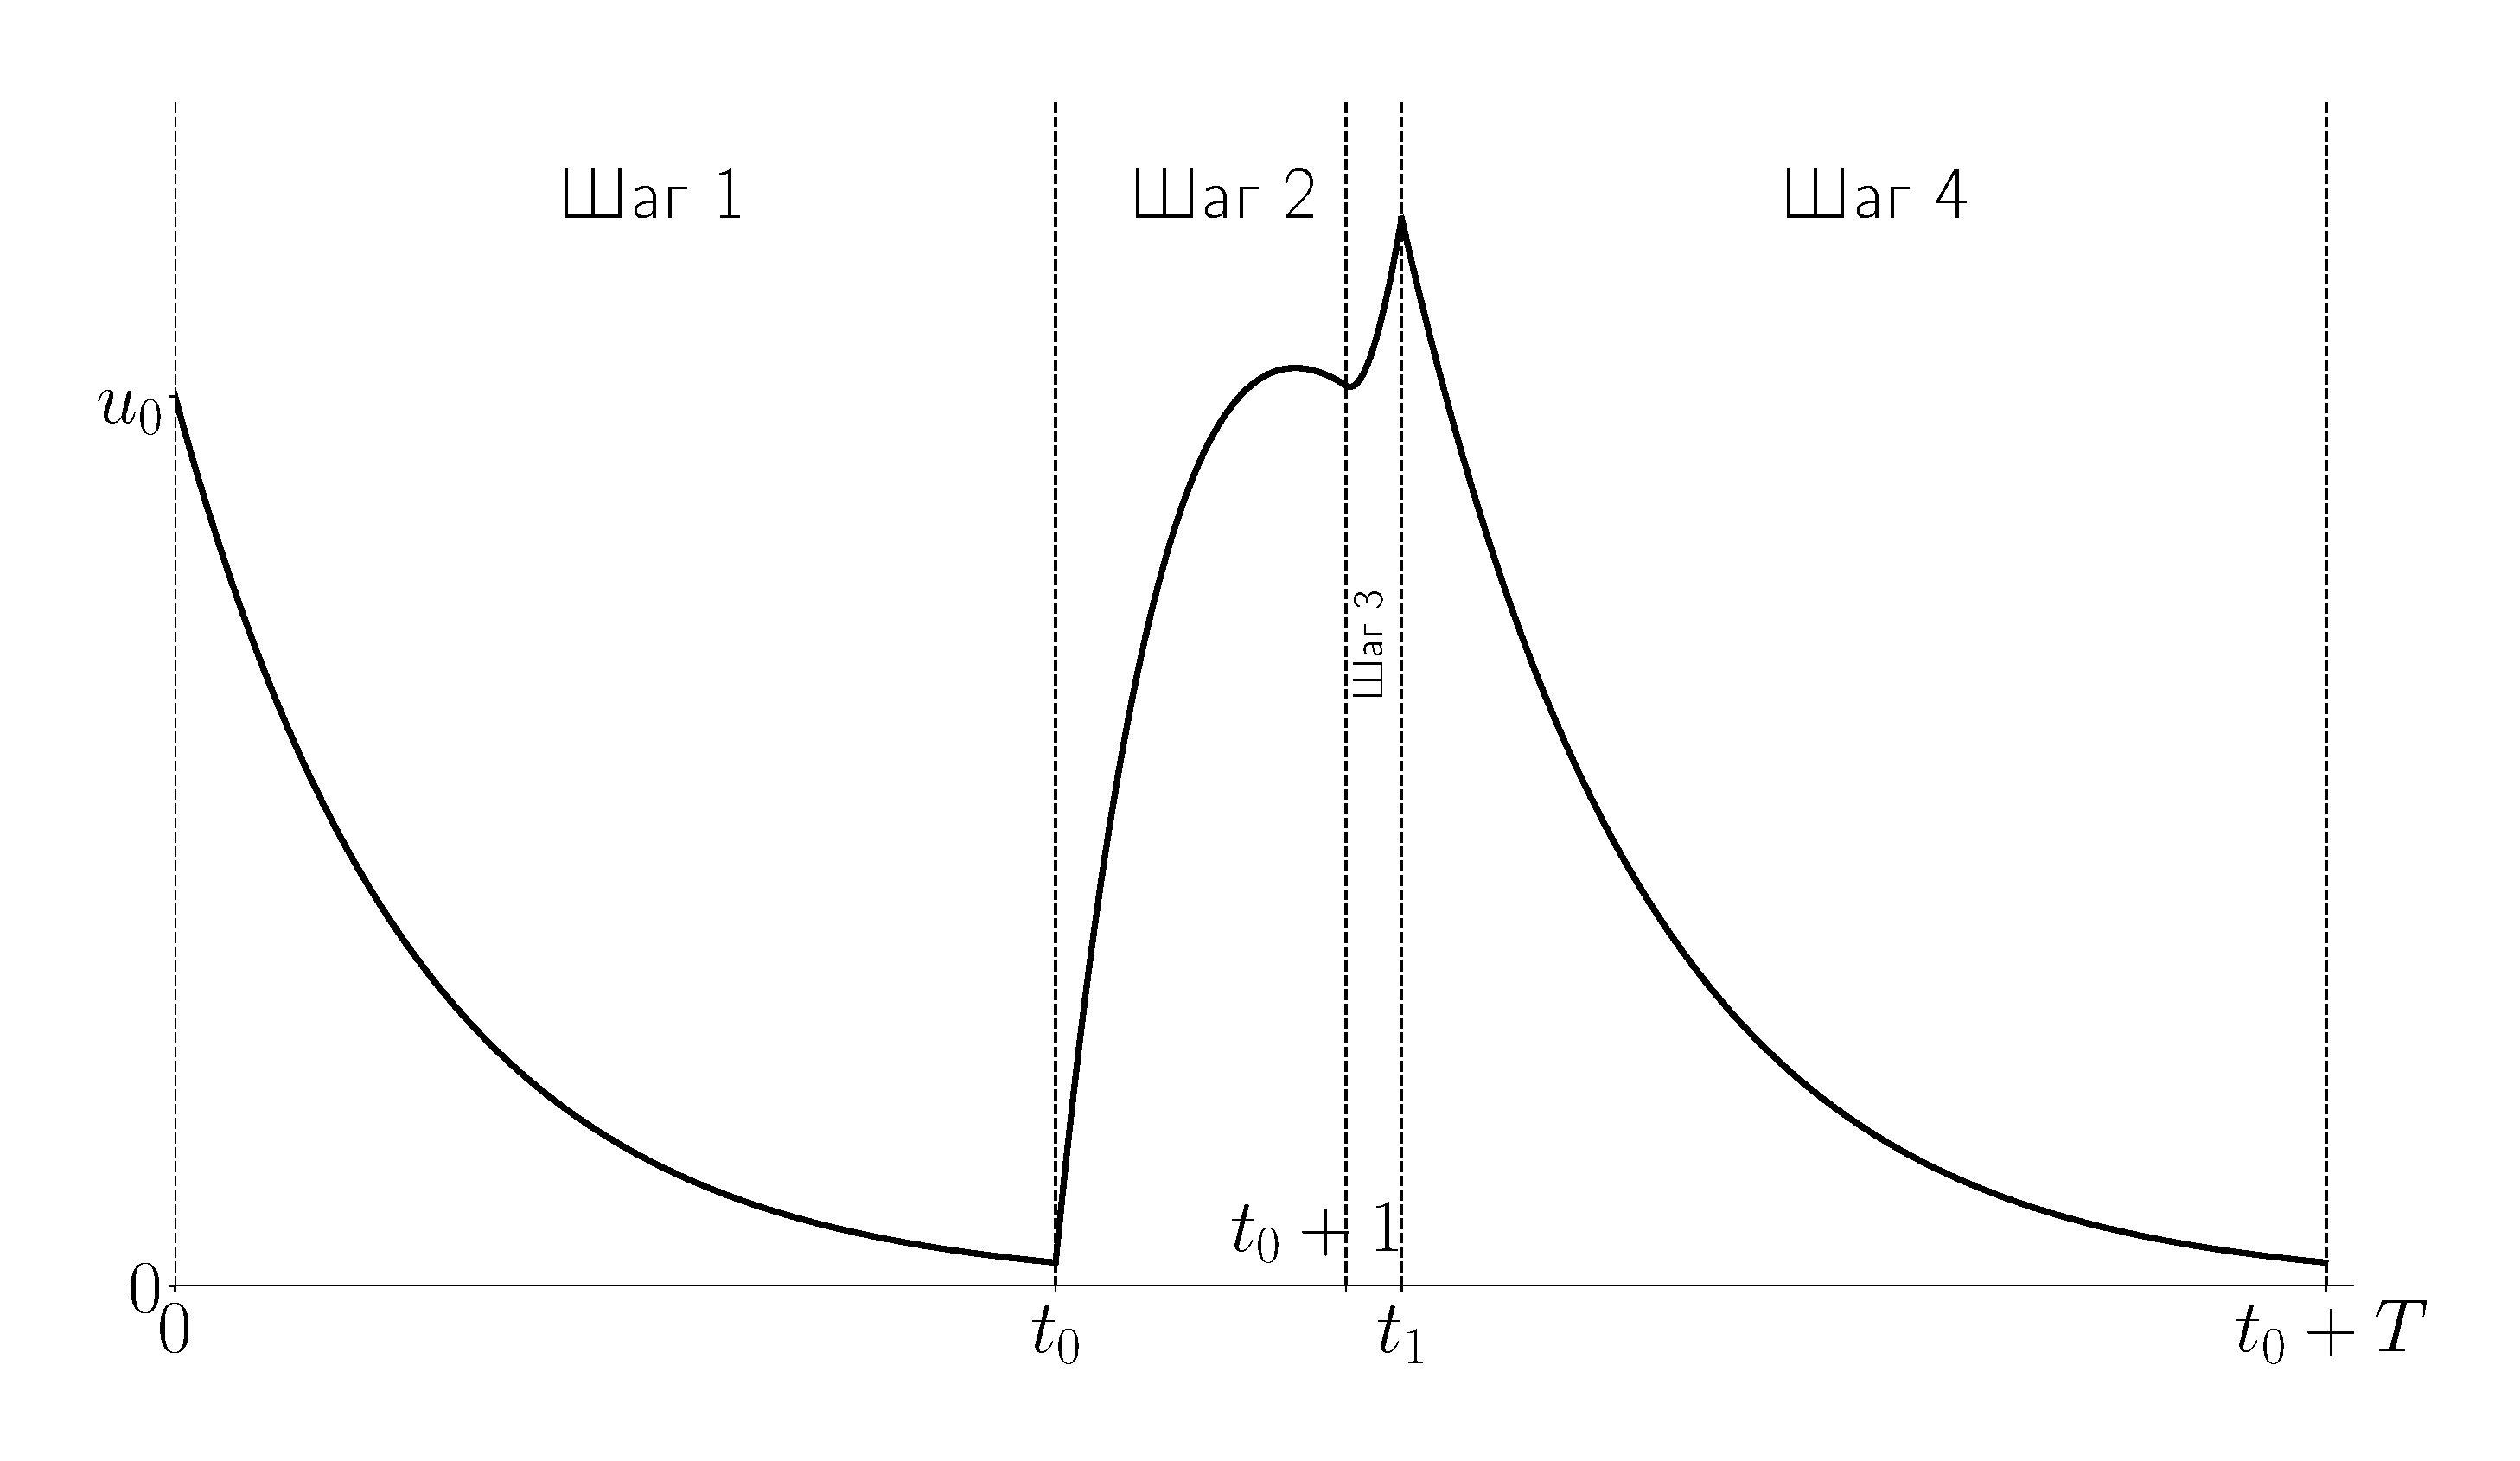
\includegraphics[width=0.7\textwidth]{u_star.eps}
	\caption{Функция $u_*(t)$, определённая на периоде $[t_0, t_0 + T]$ уравнением \eqref{eq:u_star}.}
	\label{fig:u_star}
\end{figure}

Докажем сформулированную теорему.

\subsection{Метод шагов}

Будем искать решение уравнения \eqref{eq:mg_relay_w} методом шагов, последовательно рассматривая временные отрезки между точками переключения. 

\paragraph{Шаг 1.} 
Проследим за функцией $w(t)=u(t-1)+u(t-\tau_1)+\ldots+u(t-\tau_N)$ на отрезках $[0, 1]$, $[1, \tau_1]$, \dots, $[\tau_{N-1}$, $\tau_{N}]$. Величины $t - 1$, $t - \tau_1$, \dots, $t - \tau_N$ при $t \in [0,1]$ изменяются на отрезке $[-\tau_N,0]$, а значит, здесь 
%
\begin{equation*}
	w(t)=\varphi(t-1)+\varphi(t-\tau_1)+\ldots+\varphi(t -\tau_N) > N + 1 > 1
\end{equation*}
%
и $F(w(t)) = 0$. Таким образом, 
$u(t)$ при $t\in[0,1]$ отыскивается из задачи Коши 
%
\begin{equation*}
	\dot{u}=-\beta u,\quad u(0)=u_0,
\end{equation*}
%
следовательно, описывается формулой 
%
\begin{equation*}
	u(t)=u_0e^{-\beta t}.
\end{equation*}
%
Эта формула сохранится по крайней мере на отрезке $[0, \tau_N]$, так как в $w(t)$ везде на этом промежутке входит слагаемое $\varphi(t - \tau_N) > 1$, и при переходе через точки $\tau_k$, $k = 1, \ldots, N$, слагаемое $\varphi(t-\tau_k)$ в $w(t)$ заменяется на $u_0e^{\beta (t-\tau_k)} > 0$, то есть свойство $w(t) > 1$ сохраняется. Какой бы ни была функция $\varphi\in S$, начиная с $\tau_N$, $w(t)$ имеет следующий вид, определяемый формулой $u(t)=u_0e^{-\beta t}$:
\begin{equation}
	\label{eq:w_step1}
	w(t)=u_0 e^{-\beta(t-1)} + u_0 e^{-\beta(t-\tau_1)} + \ldots + u_0 e^{-\beta(t-\tau_N)}=u_0 A e^{-\beta t}.
\end{equation} 

Формула $u(t)=u_0 e^{-\beta t}$ сохраняется до точки $t_0$, в которой $w(t)$ обращается в 1.

Таким образом, получаем, что 
\begin{equation}
	\label{eq:u_step1}
	u(t)=u_*(t)=u_0e^{-\beta t} \text{ при }t\in[0, t_0].
\end{equation}

Учитывая вид \eqref{eq:w_step1} функции $w(t)$, получаем \begin{equation}
	\label{eq:t0}
	t_0 = \frac{1}{\beta}\ln(u_0 A).
\end{equation}

Далее, начиная с точки $t_0$ в правой части уравнения \eqref{eq:mg_relay_w} величина $F(w(t))$ перестает быть нулем, поскольку аргумент становится меньше $1$. Для построения решения при $t > t_0$ докажем следующий факт.

\begin{lemma}
	\label{lm:u_star}
	На каждом шаге, пока $w(t) < 1$, функция $u(t)$ отыскивается из задачи Коши вида 
	\begin{equation}
		\label{eq:u_cauchy}
		\dot{u}=-\beta u + \alpha u_0 e^{-\beta t} P(t),\quad u(\tilde{t})=u_0 e^{-\beta \tilde{t}}\tilde{u},
	\end{equation}
	где константы $\tilde{t}$, $\tilde{u}$ и многочлен $P(t)$ определяются явно из предыдущего шага.
	Решение задачи \eqref{eq:u_cauchy} имеет вид
	\begin{equation}
		\label{eq:u_cauchy_sol}
		u(t) = u_0 e^{-\beta t}(\tilde{u}+\alpha \int_{\tilde{t}}^{t} P(s)\,ds) = u_0 e^{-\beta t} Q(t),
	\end{equation}
	где $Q(t)$ также является многочленом.
\end{lemma}

\begin{proof}
	Докажем лемму индукцией по номеру шага построения решения. На первом шаге мы имеем $P(t) \equiv 0$, $\tilde{t} = 0$, $\tilde u = 1$. Выше было показано, что в это случае решение действительно имеет вид
	%
	\begin{equation*}
		u(t) = u_0 e^{-\beta t},
	\end{equation*}
	%
	здесь $Q(t) \equiv 1$. База индукции доказана.
	
	Теперь рассмотрим задачу \eqref{eq:u_cauchy} на некотором шаге построения решения. Будем искать решение в виде
	\begin{equation}
		\label{eq:lm_ustar_cauchy}
		u(t) = u_0 e^{-\beta t} Q(t).
	\end{equation}
	%
	Подставляя в \eqref{eq:u_cauchy}, получаем
	\begin{equation*}
		\frac{d}{dt}\left(u_0 e^{-\beta t} Q(t)\right) = -\beta e^{-\beta t} u_0 Q(t) + \alpha u_0 e^{-\beta t} P(t). 
	\end{equation*}
	\begin{equation*}
		u_0 e^{-\beta t} (-\beta Q(t) + \dot{Q}(t)) = -\beta u_0 e^{-\beta t} Q(t) + \alpha u_0 e^{-\beta t} P(t).
	\end{equation*}
	\begin{equation*}
		\dot{Q}(t) = \alpha P(t).
	\end{equation*}
	Это уравнение явно интегрируется:
	\begin{equation*}
		Q(t) - Q(\tilde{t}) = \alpha \int\limits_{\tilde{t}}^t P(s)\,ds.
	\end{equation*}
	Из начальных условий задачи \eqref{eq:u_cauchy} следует, что $Q(\tilde{t}) = \tilde{u}$, откуда получаем
	\begin{equation*}
		Q(t) = \tilde{u} + \int\limits_{\tilde{t}}^t P(s)\,ds.
	\end{equation*}
	Подставляя в \eqref{eq:lm_ustar_cauchy}, получаем требуемое:
	\begin{equation*}
		u(t) = u_0 e^{-\beta t} \left(\tilde{u} + \int\limits_{\tilde{t}}^t P(s)\,ds\right),
	\end{equation*}
	где множитель в скобках действительно является полиномом от $t$.
\end{proof}

\paragraph{Шаг 2.} Следующий промежуток построения --- это отрезок  $[t_0, \min\{t_0 + 1, t_1\}]$.
Покажем, что $t_0+1 < t_1$, то есть точка переключения $t_1$ не может быть найдена на втором шаге и принадлежать отрезку $[t_0, t_0 + 1]$.
\begin{lemma}
	\label{lm:u_step2}
	$w(t)<1$ при $t \in (t_0, t_0 + 1]$.
\end{lemma}
\begin{proof}
	Рассмотрим функцию $w(t)$ на промежутке $t \in (t_0,t_0+1]$. Здесь величины $t - 1$, $t - \tau_1$, \dots, $t - \tau_N$ попадают в промежуток $(0, t_0]$, на котором $u(t)$ описывается формулой \eqref{eq:u_step1}. Это означает, что $w(t)$ описывается здесь формулой \eqref{eq:w_step1} и уравнение $w(t) = 1$ принимает вид $u_0 A e^{-\beta t} = 1$, как на первом шаге. Однако это  уравнение имеет единственный корень \eqref{eq:t0}, следовательно, $w(t) < 1$ при $t \in (t_0, t_0 + 1]$.
\end{proof}

Таким образом, следующий промежуток построения решения --- это $[t_0,t_0+1]$. Применим лемму \eqref{lm:u_star} при $P(t)\equiv A$, $\tilde{t} = t_0$, $\tilde{u} = 1$, получаем, что на отрезке $t \in [t_0, t_0 + 1]$ верно
\begin{equation}
	\label{eq:u_step2}
	u_*(t)= u_0 e^{-\beta t}\left(1 + \alpha\int\limits_{t_0}^t A\,ds \right) = u_0 e^{-\beta t}(\alpha A(t-t_0) + 1).
\end{equation}

\paragraph{Шаг 3.} Очередной промежуток построения --- это $[t_0 + 1, \min\{t_0 + \tau_*, t_1\}]$. На этом промежутке
%
\begin{multline}
	\label{eq:w3}
	w(t)=u_0 e^{-\beta (t-1)}(\alpha A(t-t_0-1)+1)+u_0 e^{-\beta(t - \tau_1)} + \ldots + u_0 e^{-\beta(t-\tau_N)} = \\
	= u_0 A e^{-\beta t}(1 + \alpha e^{\beta}(t - t_0 - 1)).
\end{multline}
Поскольку мы рассматриваем случай минимального числа точек переключения на периоде, будем считать, что $\tau_* \in (t_0 + 1, t_1)$. Условия, при которых это верно, будут сформулированы и доказаны далее.

Таким образом, следующий промежуток построения $[t_0 + 1, t_1]$. Учитывая формулу \eqref{eq:w3} и применяя лемму \ref{lm:u_star} при $P(t) = A(1 + \alpha e^\beta(t - t_0 - 1))$, $\tilde{t} = t_0+1$, $\tilde{u}=\alpha A+1$, получаем
\begin{multline}
	\label{eq:u_step3}
	u_*(t) = u_0 e^{-\beta t}\left(1 + \alpha\int\limits_{t_0 + 1}^t A(1 + \alpha A + \alpha e^\beta(s - t_0 - 1)) \,ds \right) =\\= u_0 e^{-\beta t}\left(\dfrac{\alpha^2}{2}Ae^{\beta}(t-t_0-1)^2+\alpha A(t-t_0)+1\right)\text{ при }t\in[t_0+1,t_1].
\end{multline}

\paragraph{Шаг 4.} Следующий промежуток построения функции $u(t)$ --- это $(t_1, t_2]$, на котором $w(t) > 1$. Здесь $F(w(t)) = 0$. Пусть для краткости $u_1 = u_*(t_1)$. Учитывая формулу \eqref{eq:u_step3},
\begin{equation*}
	u_1 = u(t_1) = u_0 e^{-\beta t_1}\left(\dfrac{\alpha^2}{2}Ae^{\beta}(t_1 - t_0 - 1)^2+\alpha A(t_1 - t_0)+1\right).
\end{equation*}
Тогда решение на этом промежутке находится из задачи Коши
\begin{equation*}
	\dot{u}=-\beta u,\quad u(t_1)=u_1.
\end{equation*}
Отсюда 
\begin{multline}
	\label{eq:u_step4}
	u_*(t)= u_1 e^{-\beta(t - t_1)} =\\= u_0 e^{-\beta t}\left(\dfrac{\alpha^2}{2}Ae^{\beta}(t_1 - t_0 - 1)^2 + \alpha A(t_1 - t_0) + 1\right) \text{ при } t \in (t_1,t_2].
\end{multline}

\subsection{Описание области допустимых значений параметров}

Покажем, что из условий \eqref{eq:cond_thm1}, \eqref{eq:cond_thm2} теоремы \ref{thm:mg_auxiliary_main} следует, что $t_1 \in (t_0+1,t_0+\tau_*)$.

В уравнении \eqref{eq:w3} сделаем замену $s = t - t_0$. С учётом $u_0A=e^{\beta t_0}$, получаем, что уравнение $w(t)=1$ принимает на рассматриваемом промежутке следующую форму:
\begin{equation}
	\label{eq:f}
	e^{\beta s} - \alpha e^{\beta}(s-1) - 1 = 0.
\end{equation}

Обозначим левую часть уравнения как $f(s)$. Поскольку $f''(s) = \beta^2 e^{\beta s} > 0$, функция $f(s)$ выпукла.

\begin{lemma}
	\label{lm:t1_existence}
	Существование корня $s_* > 1$ уравнения \eqref{eq:f} равносильно условию \eqref{eq:cond_thm1}.
\end{lemma}
\begin{proof}
	$f(1) = e^{\beta} - 1 > 0$. Тогда существование корня эквивалентно условию
	%
	\begin{equation*}
		\min\limits_{s > 1}f(s) < 0.
	\end{equation*}
	
	Найдём точку минимума $s_{\min}$ функции $f(s)$.
	\begin{equation*}
		f'(s) = 0 \ \Leftrightarrow \ \beta e^{\beta s} - \alpha e^{\beta} = 0\ \Leftrightarrow\ s = 1 + \frac{1}{\beta}\ln\frac{\alpha}{\beta}.
	\end{equation*}
	Поскольку $f(s)$ выпукла, это действительно точка минимума. Подставим её в условие $f(s_{\min}) < 0$:
	\begin{equation*}
		\exp\left(\beta (1 + \frac{1}{\beta}\ln\frac{\alpha}{\beta}) \right) - \alpha e^{\beta}(1 + \frac{1}{\beta}\ln\frac{\alpha}{\beta} - 1) - 1 < 0 \Leftrightarrow
	\end{equation*}
	\begin{equation*}
		\frac{\alpha}{\beta}e^{\beta}\left(1 + \ln\frac{\beta}{\alpha}\right) < 1,
	\end{equation*}
	что соответствует первой части условия \eqref{eq:cond_thm1}.
	
	Если $s_{\min} < 1$, то корень уравнения \eqref{eq:f} также будет меньше $1$ (в случае существования). Поэтому условию $s_* > 1$ соответствует ограничение $s_{\min} > 1$:
	\begin{equation*}
		1 + \frac{1}{\beta}\ln\frac{\alpha}{\beta} > 1 \quad \Leftrightarrow \quad \alpha > \beta.
	\end{equation*}
\end{proof}

\begin{lemma}
	\label{lm:t1_locate}
	Пусть выполнены условия леммы \ref{lm:t1_existence}. Корень $s_*$ уравнения \eqref{eq:f} (меньший, если их два) принадлежит промежутку $(1,\tau_*]$ тогда и только тогда, когда выполняется хотя бы одно из двух условий:
	\begin{enumerate}
		\item[1)] $e^{\beta \tau_*} - 1 \leqslant \alpha e^\beta(\tau_* - 1)$,
		\item[2)] $0 < \frac{1}{\beta}\ln\frac{\alpha}{\beta}\leqslant\tau_*-1$.
	\end{enumerate}
\end{lemma}
\begin{proof}
	Поскольку $f(1) > 0$, возможны две ситуации: $f(\tau_*) \leqslant 0$ или $f(\tau_*) > 0$, но $s_{\min} \leq \tau_*$, см. рисунок \ref{fig:tau_star}.

\begin{figure}[ht]
	\centering
	\begin{minipage}{.45\linewidth}
		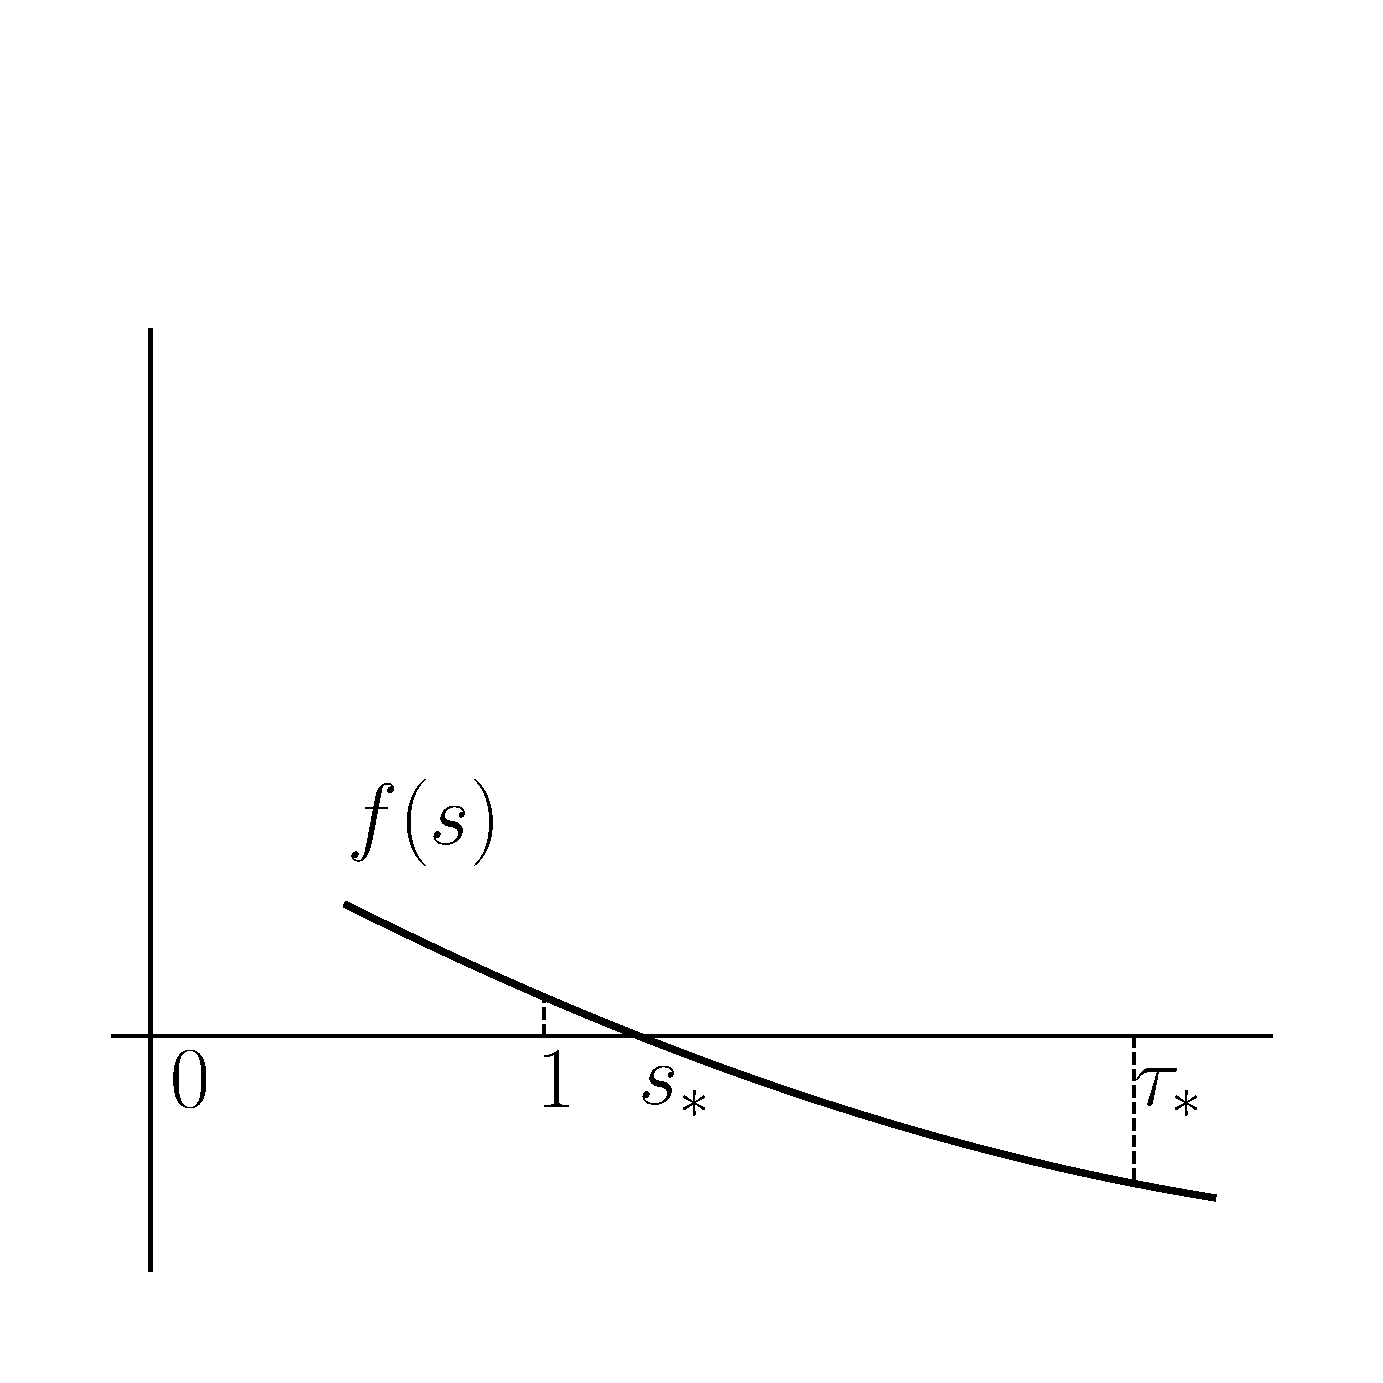
\includegraphics[width=\linewidth]{images/f2.eps}
	\end{minipage}
	\hspace{.05\linewidth}
	\begin{minipage}{.45\linewidth}
		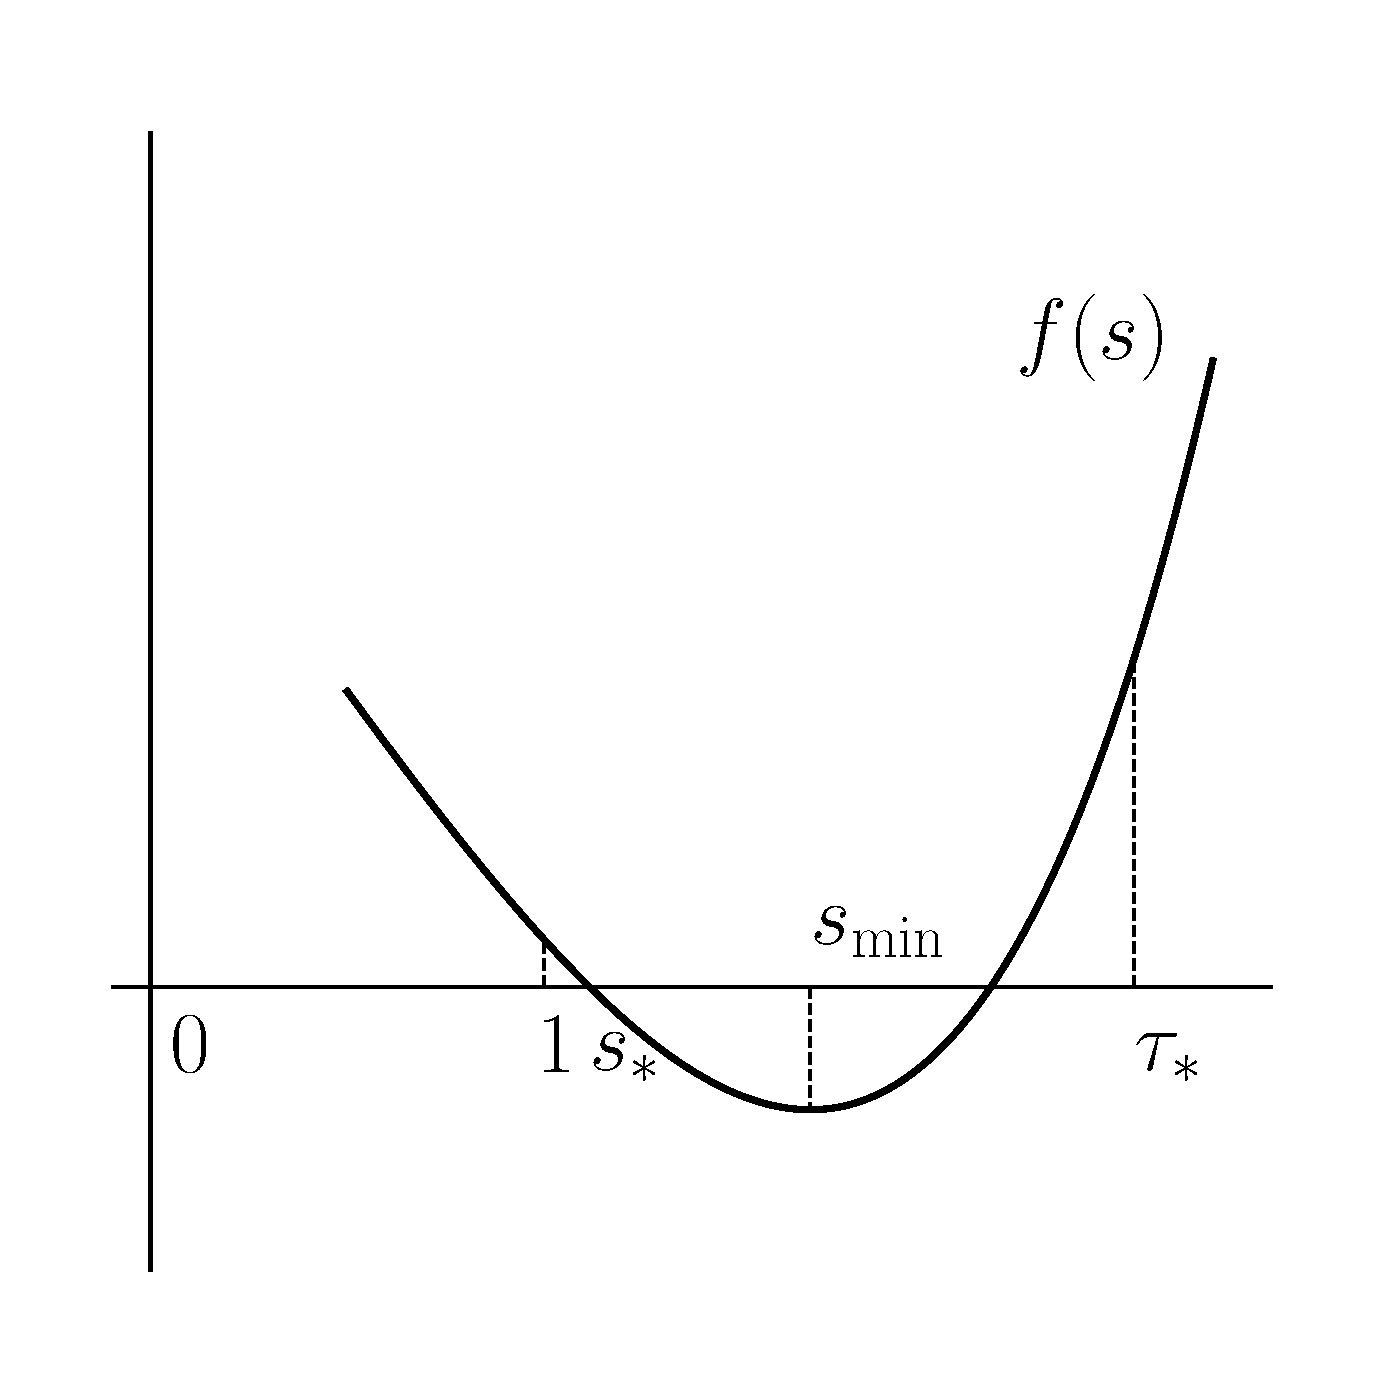
\includegraphics[width=\linewidth]{images/f1.eps}
	\end{minipage}
	\caption{Варианты взаимного расположения графика функции $f(s)$ при условии, что корень $s_*$ уравнения \eqref{eq:f} существует и попадает на интервал $(1,\tau_*)$. На левом изображении $f(1) > 0$ и $f(\tau_*) \leq 0$. На правом рисунке $f(1) > 0$ и $f(\tau_*) > 0$, но точка минимума $s_{\min}$ принадлежит промежутку $(1,\tau_*]$.}
	\label{fig:tau_star}
\end{figure}

Случай $f(\tau_*) \leq 0$ соответствует условию 1), случай $1 < s_{\min} \leqslant \tau_*$ --- условию 2) леммы. 
\end{proof}

Таким образом, мы доказали, что из условий \eqref{eq:cond_thm1} и \eqref{eq:cond_thm2} теоремы \ref{thm:mg_auxiliary_main} следует, что корень $s_*$ уравнения \eqref{eq:f} существует и лежит между $1$ и $\tau_*$. Это означает, что точка переключения $t_1 = t_0 + s_*$ также существует и попадает на отрезок $[t_0 + 1, t_0 + \tau_*]$.

Далее мы опишем область значений параметров, удовлетворяющих условиям \eqref{eq:cond_thm1} и \eqref{eq:cond_thm2} явно.

Выразим $\alpha$ из условия \eqref{eq:cond_thm1}.
\begin{equation*}
\frac{\alpha}{\beta}e^{\beta}\left(\ln\frac{\beta}{\alpha} + 1\right) \leqslant 1\ \Leftrightarrow\ 1 + \ln\dfrac{\beta}{\alpha} \leqslant \dfrac{\beta e^{-\beta}}{\alpha}.
\end{equation*}

Возьмём экспоненту от обеих частей:
\begin{equation*}
\dfrac{e\beta}{\alpha} \leqslant \exp\dfrac{\beta e^{-\beta}}{\alpha}\ \Leftrightarrow\ \dfrac{-\beta e^{-\beta}}{\alpha}\exp \dfrac{-\beta e^{-\beta}}{\alpha} \geqslant -e^{-\beta - 1}\ \Leftrightarrow
\end{equation*}

\begin{align}
\label{eq:step3_cond1_expanded}
\left[
\begin{array}{ll}
	-\frac{\beta e^{-\beta}}{\alpha} \geqslant W_0(-e^{-\beta - 1}),\\
	-\frac{\beta e^{-\beta}}{\alpha} \leqslant W_{-1}(-e^{-\beta - 1}).
\end{array}
\right.
\end{align}
%
где $W_0(x)$ --- ветвь W-функции Ламберта, определённая при $x \in [-1; +\infty)$, а $W_{-1}(x)$ --- ветвь, определённая при $x \in (-\infty; -1]$.

Однако, второе неравенство соответствует случаю $\dfrac{-\beta e^{-\beta}}{\alpha} < -1$ (поскольку $W_{-1}(x)$ определена при $x < -1$). Тогда
\begin{equation*}
\alpha < \beta e^{-\beta} < \beta,
\end{equation*}
что противоречит условию \eqref{eq:cond_thm1}.

Значит, в совокупности неравенств \eqref{eq:step3_cond1_expanded} заменяется на единственное неравенство
\begin{equation}
\label{eq:step3_cond1}
-\frac{\beta e^{-\beta}}{\alpha} \geqslant W(-e^{-\beta - 1})
\end{equation}
Здесь и далее, будем писать $W$ вместо $W_0$ для обозначения соответствующей ветви функции Ламберта.

Определим функцию
\begin{equation}
\label{eq:step_3_phi_func}
\varphi(\beta) = - \dfrac{\beta e^{-\beta}}{W_0(-e^{-\beta - 1})}.
\end{equation}
%
В этих обозначениях условие \eqref{eq:step3_cond1} перепишется как
%
\begin{equation}
\label{eq:step_3_cond_phi}
\alpha \geqslant \varphi(\beta).
\end{equation}

Теперь выразим $\alpha$ из условия \eqref{eq:cond_thm2}:
\begin{equation}
\label{eq:step3_cond2_expanded_1}
e^{\beta \tau_*}-1\leqslant\alpha e^\beta(\tau_*-1)\ \Leftrightarrow\ \alpha \geqslant \dfrac{e^{\beta \tau_*}-1}{e^\beta(\tau_*-1)}.
\end{equation}
\begin{equation}
\label{eq:step3_cond2_expanded_2}
\frac{1}{\beta}\ln\frac{\alpha}{\beta}\leqslant\tau_*-1\ \Leftrightarrow\ \alpha \leqslant \beta e^{\beta (\tau_* - 1)}.
\end{equation}

Определим функции
\begin{equation}
\label{eq:step_3_theta_func}
\theta(\beta, \tau_*) = \dfrac{e^{\beta \tau_*}-1}{e^\beta(\tau_*-1)}.
\end{equation}
%
\begin{equation}
\label{eq:step_3_psi_func}
\delta(\beta, \tau_*) = \beta e^{\beta (\tau_* - 1)}.
\end{equation}
%
В этих обозначениях условие \eqref{eq:cond_thm2} перепишется как
%
\begin{equation}
\label{eq:step_3_cond_2}
\left[
\begin{array}{ll}
	\alpha \geqslant \theta(\beta, \tau_*),\\
	\alpha \leqslant \delta(\beta, \tau_*).
\end{array}
\right.
\end{equation}

Исследуем взаимное расположение функций $\phi$, $\theta$ и $\delta$.

\begin{lemma}
\label{lm:tau_star_sol}
Уравнение 
\begin{equation}
	e^{\beta x}(\beta(x - 1) - 1) + 1 = 0.
\end{equation}
при фиксированном $\beta > 0$ имеет единственный корень, больший единицы:
\begin{equation}
	x = 1 + \frac{1 + W(-e^{-\beta - 1})}{\beta}.
\end{equation}
\end{lemma}
\begin{proof}

\begin{multline*}
	e^{\beta x}(\beta(x - 1) - 1) = -1 \Leftrightarrow e^{\beta(x - 1) - 1}(\beta(x - 1) - 1) = -e^{-\beta - 1}\ \Leftrightarrow\\\Leftrightarrow\ \beta(x - 1) - 1 = W(-e^{-\beta - 1})\ \Leftrightarrow\ x = 1 + \dfrac{1 + W(-e^{-\beta - 1})}{\beta}.
\end{multline*}

Здесь применение функции $W$ корректно, поскольку $\beta(x - 1) - 1 > -1$ и $-e^{-\beta - 1} > -\frac{1}{e}$.

\end{proof}


\begin{lemma}
	\label{lm:beta_tilde_sol}
	Уравнение 
	\begin{equation*}
		e^{\beta x}(\beta(x - 1) - 1) + 1 = 0.
	\end{equation*}
	при фиксированном $x > 1$ имеет единственный положительный корень:
	\begin{equation*}
		\tilde{\beta}(x) = \frac{1}{x - 1} + \frac{1}{x}W\left(\frac{x}{1 - x} e^{\frac{x}{1 - x}}\right).
	\end{equation*}
\end{lemma}

\begin{proof}
	Перенесём единицу в правую часть:
	%
	\begin{equation*}
		e^{\beta x}(\beta(x - 1) - 1) = -1.
	\end{equation*}
	%
	Домножим на $\frac{x}{x - 1}$:
	%
	\begin{equation*}
		e^{\beta x}\left( \beta x + \frac{x}{x - 1} \right) = -\frac{x}{x - 1}. 
	\end{equation*}
	%
	Домножим обе части уравнения на $e^{\frac{x}{x - 1}}$:
	%
	\begin{equation*}
		\left( \beta x - \frac{x}{1 - x} \right) e^{\beta x - \frac{x}{1 - x}} = \frac{x}{1 - x} e^{\frac{x}{1 - x}}. 
	\end{equation*}
	%
	Функция $f(t) = t e^t$ принимает значение $\frac{x}{1 - x} e^{\frac{x}{1 - x}}$ ровно в двух точках: $t = \frac{x}{1 - x} < -1$ и $t = W\left(\frac{x}{1 - x} e^{\frac{x}{1 - x}}\right) \in (-1; 0)$.
	
	\begin{align*}
		\left[
		\begin{array}{ll}
			\beta x + \frac{x}{1 - x} = \frac{x}{1 - x};\\
			\beta x + \frac{x}{1 - x} = W\left(\frac{x}{1 - x} e^{\frac{x}{1 - x}}\right).
		\end{array}
		\right.
	\end{align*}
	
	Первое равенство при допустимых значениях параметров не имеет решений, второе даёт единственное решение
	\[
	\beta = \frac{1}{x - 1} + \frac{1}{x} W\left(\frac{x}{1 - x} e^{\frac{x}{1 - x}}\right).
	\]
\end{proof}

\begin{proposition}
	\label{prop:phi_theta}
	$\phi(\beta) = \min\limits_{\tau_* > 1} \theta(\beta, \tau_*)$.
\end{proposition}

\begin{proof}
	\begin{equation*}
		\frac{d}{d\tau_*} \theta(\beta, \tau_*) = \frac{d}{d\tau_*} \left( \frac{e^{\beta\tau_*} - 1}{e^{\beta}(\tau_* - 1)} \right) = \frac{e^{-\beta}\left(e^{\beta \tau_*}(\beta(\tau_* - 1) - 1) + 1\right)}{(\tau_* - 1)^2}.
	\end{equation*}
	Нуль производной соответствует решению уравнения
	\begin{equation*}
		e^{\beta \tau_*}(\beta(\tau_* - 1) - 1) + 1 = 0
	\end{equation*}
	относительно $\tau_*$. По лемме \ref{lm:tau_star_sol}, такое решение существует и единственно при $\tau_* > 1$, обозначим его
	\begin{equation*}
		\tau_*^{\min} = 1 + \frac{1 + W(-e^{-\beta - 1})}{\beta}.
	\end{equation*}
	Заметим, что оно действительно будет точкой минимума функции $ \theta(\beta, \tau_*)$ при фиксированном $\beta$, поскольку
	\begin{equation*}
		\lim\limits_{\tau_* \to 1 + 0} \theta(\beta, \tau_*) = \lim\limits_{\tau_* \to +\infty} \theta(\beta, \tau_*) = +\infty. 
	\end{equation*}
	
	Из условия
	\begin{equation*}
		e^{\beta \tau_*^{\min}}(\beta(\tau_*^{\min} - 1) - 1) + 1 = 0
	\end{equation*}
	выразим $e^{\beta \tau_*^{\min}} - 1$:
	\begin{equation*}
		e^{\beta \tau_*^{\min}} - 1 = \beta e^{\beta \tau_*^{\min}} (\tau_*^{\min} - 1)
	\end{equation*}
	и подставим в функцию $\theta(\beta, \tau_*)$:
	\begin{multline}
		\theta(\beta, \tau_*^{\min}) = \frac{e^{\beta\tau_*^{\min}} - 1}{e^{\beta}(\tau_*^{\min} - 1)} = \frac{\beta e^{\beta \tau_*^{\min}} (\tau_*^{\min} - 1)}{e^{\beta}(\tau_*^{\min} - 1)} =\\= \beta e^{\beta (\tau_*^{\min} - 1)} = \beta e^{\beta(1 + \frac{1 + W(-e^{-\beta - 1})}{\beta} - 1)} = \beta e^{1 + W(-e^{-\beta - 1})}. 
	\end{multline}
	
	Теперь убедимся, что $\theta(\beta, \tau_*^{\min}) = \phi(\beta)$.
	%
	\begin{equation*}
		\beta e^{1 + W(-e^{-\beta - 1})} = -\frac{\beta e^{-\beta}}{W(-e^{-\beta - 1})} \Leftrightarrow -e^{-\beta - 1} = W(-e^{-\beta - 1}) e^{W(-e^{-\beta - 1})},
	\end{equation*}
	что является верным равенством, поскольку $-e^{-\beta - 1} > -\frac{1}{e}$.
\end{proof}


\begin{proposition}
	\label{prop:delta_theta}
	$\delta(\beta, \tau_*) \geq \theta(\beta, \tau_*) \Leftrightarrow \beta \geq \tilde{\beta}(\tau_*)$ при $\beta > 0$, $\tau_* > 1$.  
\end{proposition}

\begin{proof}
	Решим относительно $\beta$ уравнение 
	\[
	\delta(\beta, \tau_*) = \theta(\beta, \tau_*).
	\]
	\[
	\beta e^{\beta(\tau_*- 1)} = \dfrac{e^{\beta \tau_*} - 1}{e^{\beta} (\tau_* - 1)} \Leftrightarrow e^{\beta\tau_*}(\beta(\tau_* - 1) - 1) = -1.
	\]
	По лемме \ref{lm:beta_tilde_sol}, единственное решение этого уравнения $\beta = \tilde{\beta}(\tau_*)$.
	
	При $\beta \to +\infty$ функция $\theta(\beta, \tau_*) \sim \frac{1}{\tau_* - 1}e^{\beta(\tau_* - 1)}$ асимптотически меньше, чем $\delta(\beta, \tau_*) = \beta e^{\beta (\tau_* - 1)}$. Из непрерывности следует, что при $\beta > \tilde{\beta}(\tau_*)$ верно неравенство
	\[
	\delta(\beta, \tau_*) > \theta(\beta, \tau_*).
	\]
	
	Теперь сравним функции при малых значениях $\beta > 0$. Заметим, что $\theta(0, \tau_*) = \delta(0, \tau_*) = 0$.
	\[
	\frac{d}{d\beta}\theta(\beta, \tau_*)\Bigg\vert_{\beta = 0} = e^{-\beta}\left( e^{\beta \tau_*} + \frac{1}{\tau_* - 1}\right)\Bigg\vert_{\beta = 0} = 1 + \frac{1}{\tau_* - 1} > 1;
	\]
	\[
	\frac{d}{d\beta}\delta(\beta, \tau_*)\Bigg\vert_{\beta = 0} = e^{\beta(\tau_* - 1)}(\beta(\tau_* - 1) + 1)\Bigg\vert_{\beta = 0} = 1.
	\]
	Поскольку
	\[
	\frac{d}{d\beta}\delta(\beta, \tau_*)\bigg\vert_{\beta = 0} < \frac{d}{d\beta}\theta(\beta, \tau_*)\bigg\vert_{\beta = 0},
	\]
	при малых значениях $\beta > 0$ выполнено неравенство
	\[
	\delta(\beta, \tau_*) < \theta(\beta, \tau_*),
	\]
	а из непрерывности оно распространяется на весь промежуток $\left(0, \tilde{\beta}(\tau_*)\right)$.    
\end{proof}


\begin{proposition}
	\label{prop:delta_phi}
	$\delta(\beta, \tau_*) \geq \phi(\beta) \Leftrightarrow \beta \geq \tilde{\beta}(\tau_*)$ при $\beta > 0$, $\tau_* > 1$.  
\end{proposition}

\begin{proof}
	Решим относительно $\beta$ неравенство 
	\[
	\delta(\beta, \tau_*) = \phi(\beta).
	\]
	\[
	-\dfrac{\beta e^{-\beta}}{W(-e^{-\beta - 1})} \geqslant \beta e^{\beta(\tau_* - 1)}\ \Leftrightarrow\ W(-e^{-\beta - 1}) \geqslant -e^{-\beta\tau_*}
	\]
	%
	Поскольку $-e^{-\beta - 1} \geqslant -e^{-1}$ и $-e^{-\beta\tau_*} \geqslant -1$, преобразование $x \mapsto x e^x$ является монотонным и взаимно однозначным.
	%
	\begin{multline*}
		-e^{-\beta - 1} \geqslant -e^{-\beta\tau_*}\exp(-e^{-\beta\tau_*})\ \Leftrightarrow\ e^{-\beta - 1 + \beta\tau_*} \leqslant \exp(-e^{-\beta\tau_*})\ \Leftrightarrow
		\\
		\Leftrightarrow\ -\beta - 1 + \beta\tau_* \leqslant -e^{-\beta \tau_*}\ \Leftrightarrow \ e^{\beta \tau_*}(\beta(\tau_* - 1) - 1) \leqslant -1\ \Leftrightarrow
		\\
		\Leftrightarrow\ \left(\beta \tau_* + \frac{\tau_*}{1 - \tau_*}\right) e^{\beta \tau_* + \frac{\tau_*}{1 - \tau_*}} \leqslant \frac{\tau_*}{1 - \tau_*} e^{\frac{\tau_*}{1 - \tau_*}}.
	\end{multline*}
	%
	Функция $f(x) = x e^x$ принимает значение $\frac{\tau_*}{1 - \tau_*} e^{\frac{\tau_*}{1 - \tau_*}}$ ровно в двух точках: $x = \frac{\tau_*}{1 - \tau_*} < -1$ и $x = W\left(\frac{\tau_*}{1 - \tau_*} e^{\frac{\tau_*}{1 - \tau_*}}\right) \in (-1; 0)$.
	
	Тогда равносильным будет переход к следующему неравенству (см. рис. \ref{fig:w_inverse}):
	\begin{equation}
		\label{eq:phi_double_inequality}
		\frac{\tau_*}{1 - \tau_*} \leqslant \beta \tau_* + \frac{\tau_*}{1 - \tau_*} \leqslant  W\left(\frac{\tau_*}{1 - \tau_*} e^{\frac{\tau_*}{1 - \tau_*}}\right).
	\end{equation}
	%
	Левая часть эквивалентна $\beta \geqslant 0$, а правая $\beta \leqslant \tilde{\beta}(\tau_*)$.
	%
	\begin{figure}[ht]
		\centering
		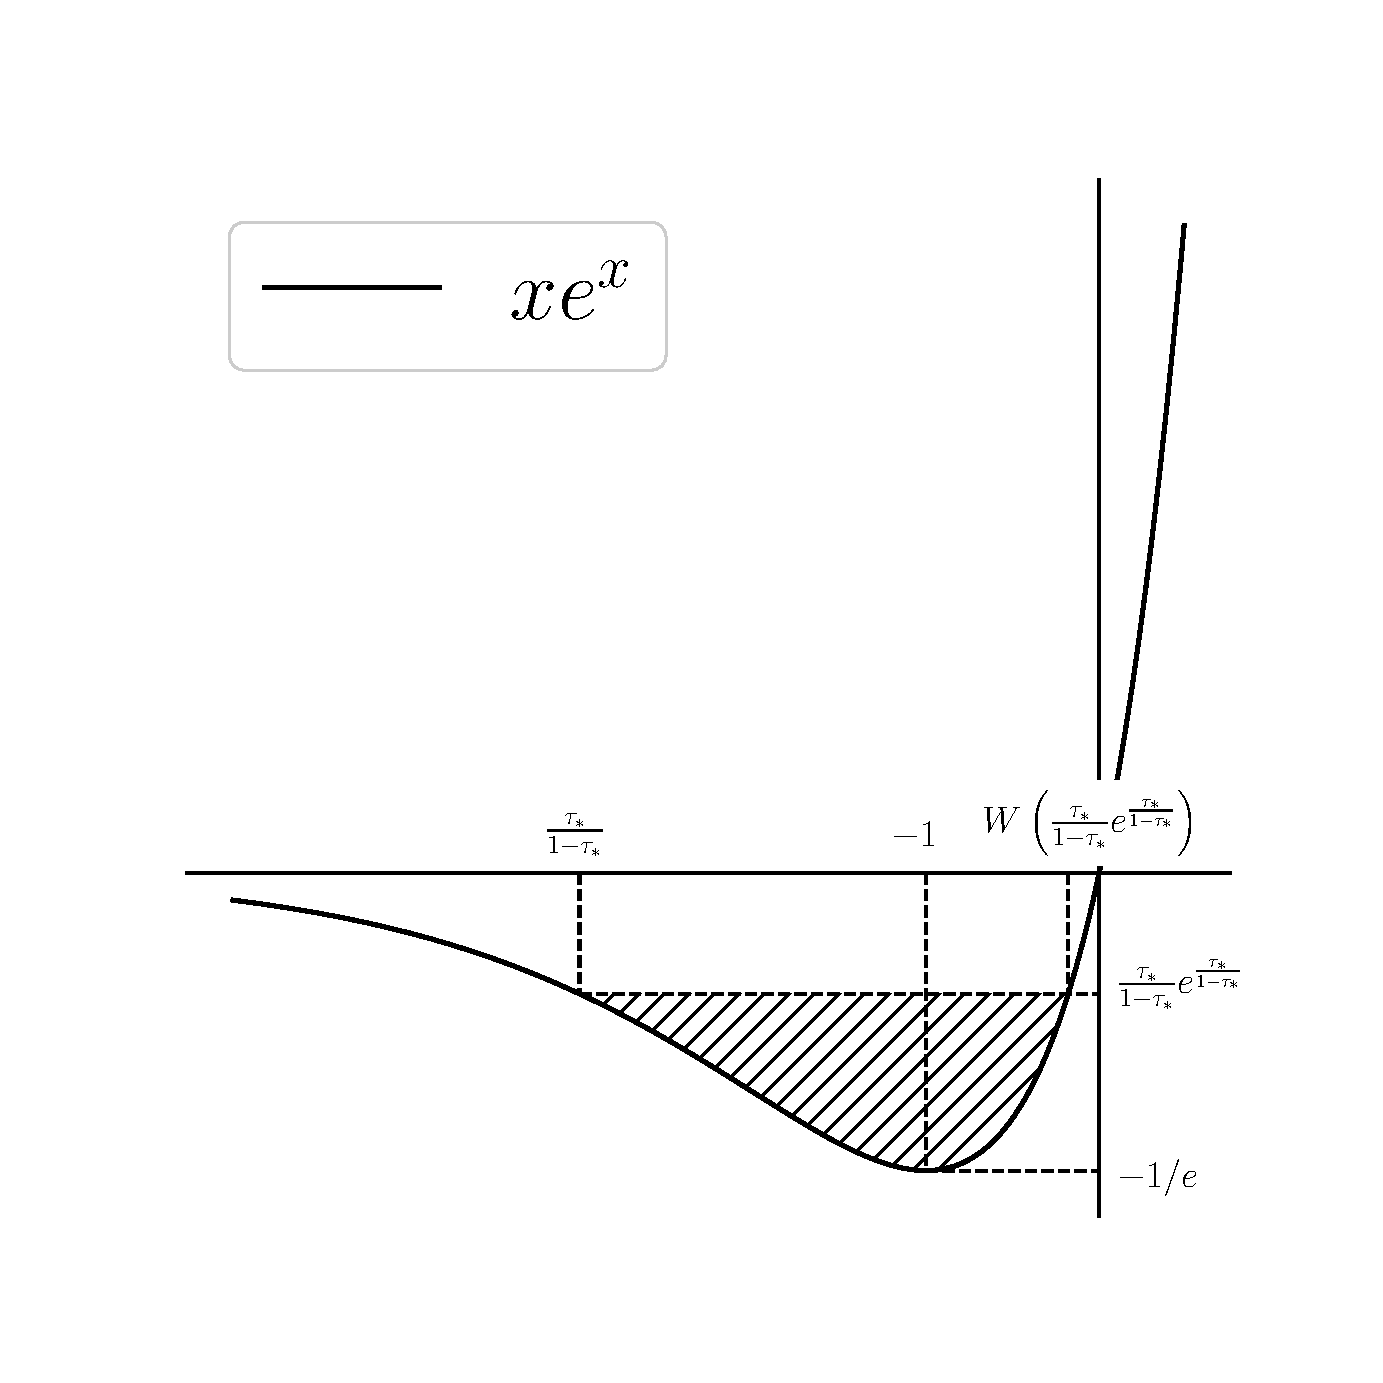
\includegraphics[width=0.7\textwidth]{w_inverse.eps}
		\caption{Функция $f(x) = x e^x$ убывает при $x < -1$ и возрастает при $x > -1$. На рисунке изображена область, соответствующая неравенству \eqref{eq:phi_double_inequality}.}
		\label{fig:w_inverse}
	\end{figure}
	
	Также заметим, что равенство выполняется только в точке $\beta = \tilde{\beta}(\tau_*)$.
	
\end{proof}

Теперь проанализируем условия \eqref{eq:step_3_cond_phi} и \eqref{eq:step_3_cond_2}. По утверждениям \ref{prop:phi_theta}, \ref{prop:delta_theta} и \ref{prop:delta_phi},
\begin{equation}
	\begin{cases}
		\delta(\beta, \tau_*) < \phi(\beta) < \theta(\beta, \tau_*), & \beta < \tilde{\beta}(\tau_*),\\
		\delta(\beta, \tau_*) = \phi(\beta) = \theta(\beta, \tau_*), & \beta = \tilde{\beta}(\tau_*),\\
		\delta(\beta, \tau_*) > \theta(\beta, \tau_*) > \phi(\beta), & \beta > \tilde{\beta}(\tau_*).
	\end{cases}
\end{equation}
%
Тогда условия \eqref{eq:step_3_cond_phi} и \eqref{eq:step_3_cond_2} можно представить в упрощённом виде:
\begin{equation}
	\label{eq:phi_theta_cond}
	\begin{cases}
		\alpha \geq \theta(\beta, \tau_*), & \beta \leq \tilde{\beta}(\tau_*),\\
		\alpha \geq \phi(\beta), & \beta > \tilde{\beta}(\tau_*).
	\end{cases}
\end{equation}


На рисунке \ref{fig:step3_t1} изображена область параметров для различных фиксированных значений $\tau_*$.

\begin{figure}
	\centering
	\begin{minipage}{.45\linewidth}
		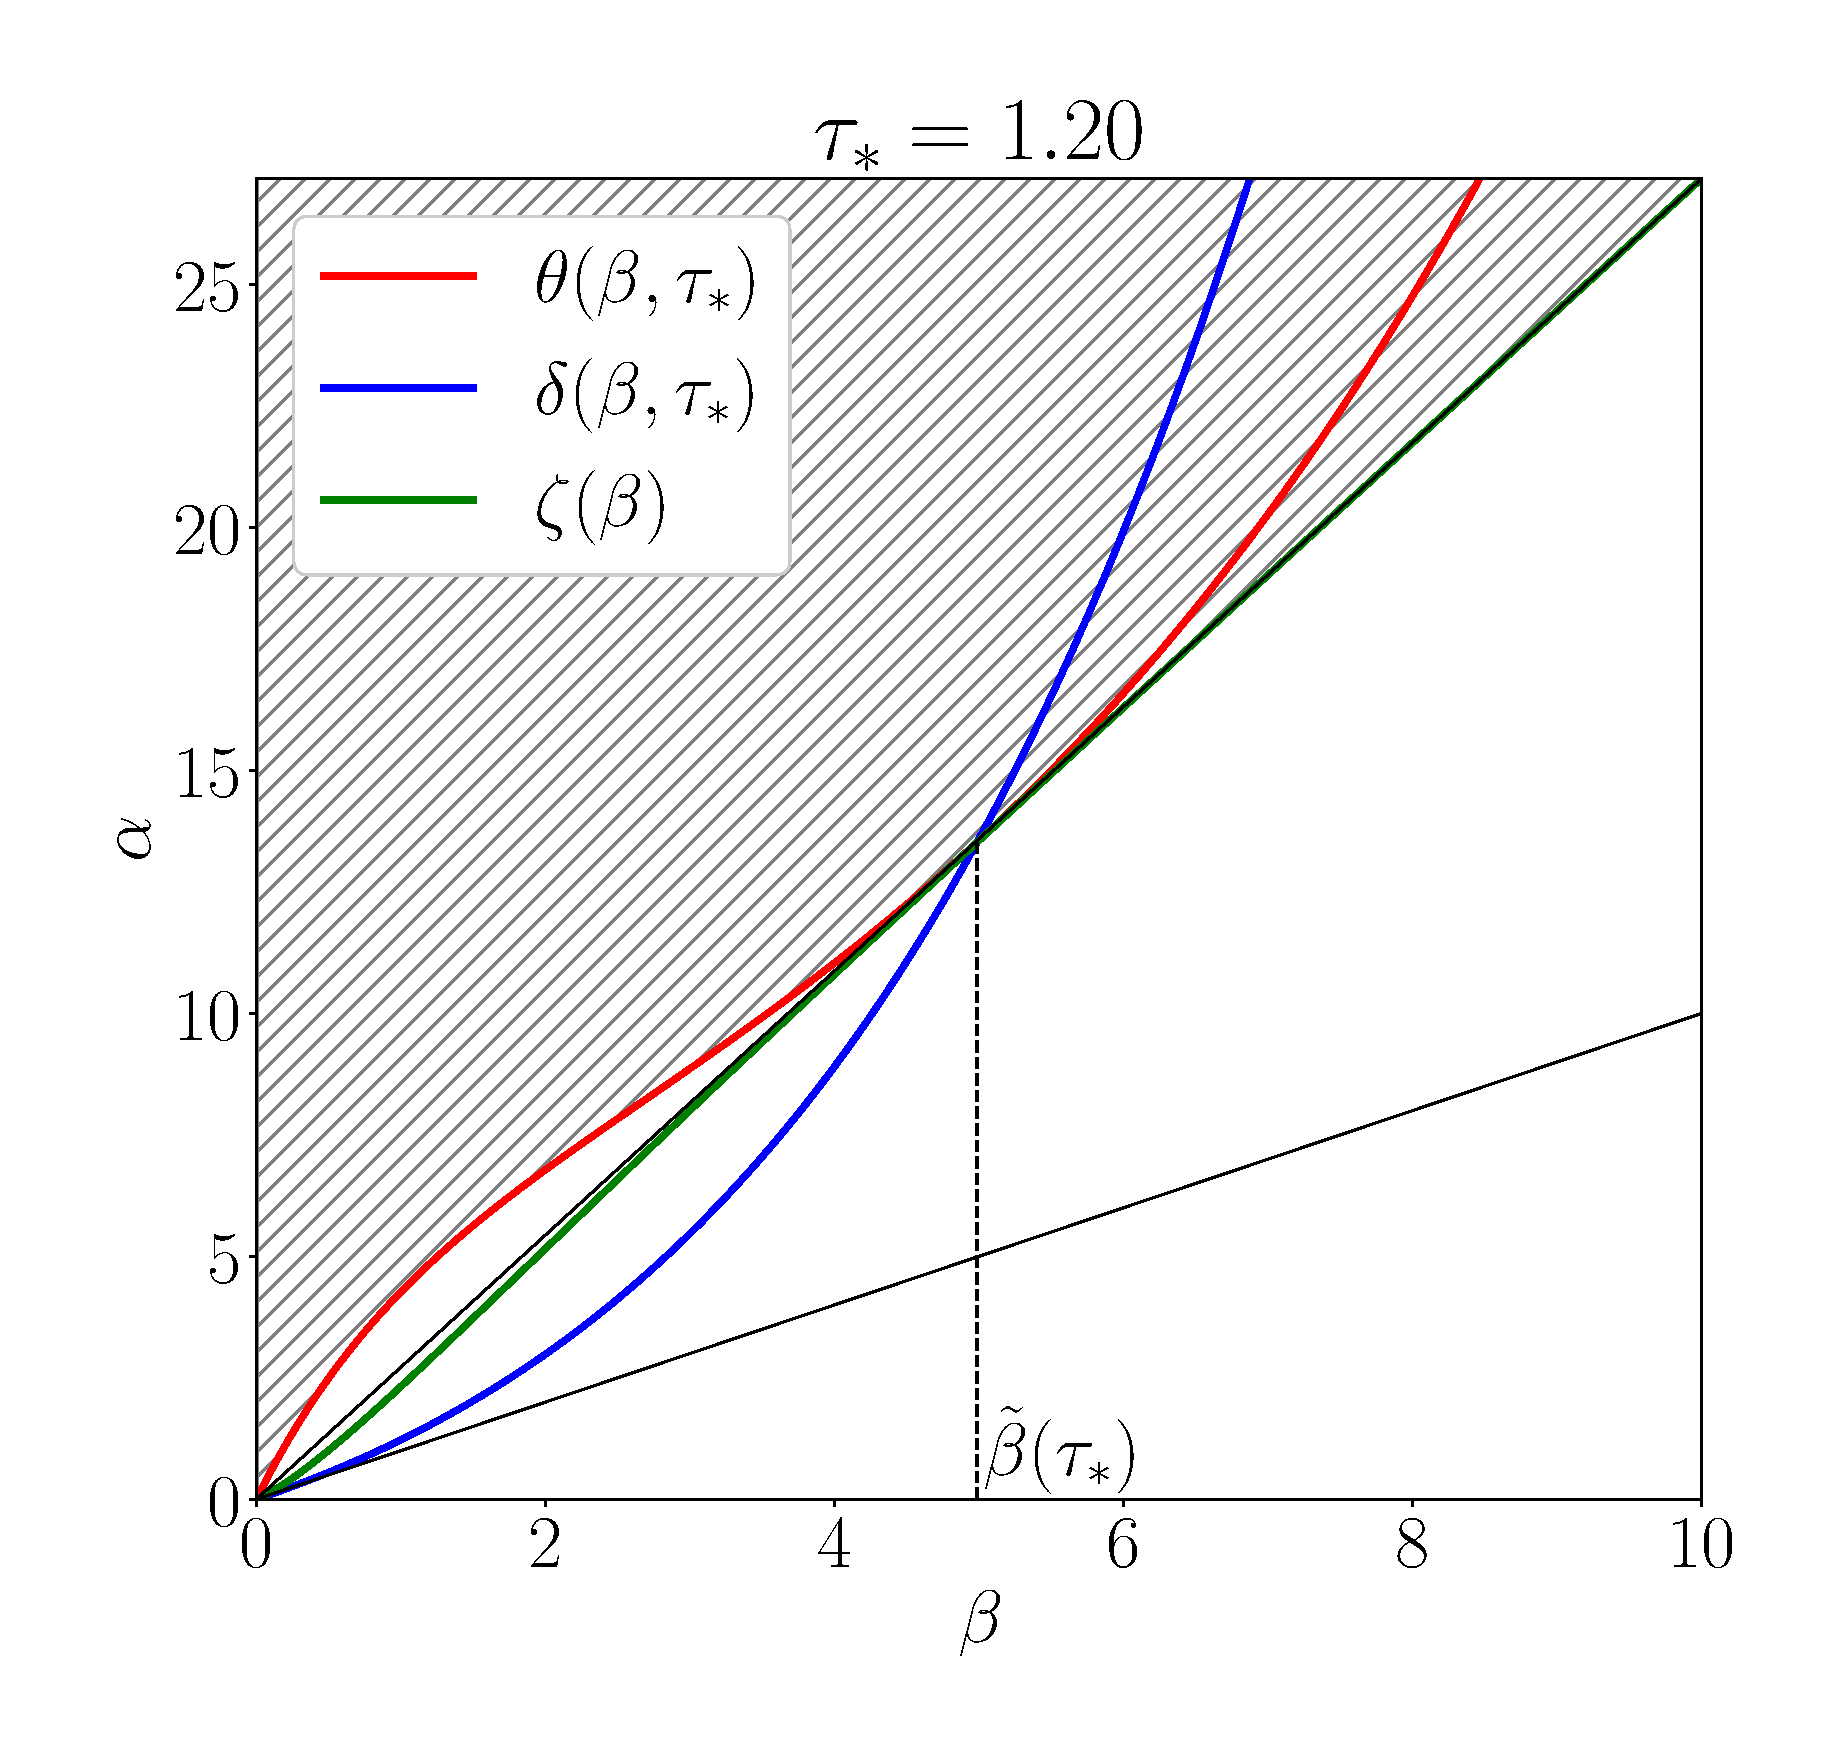
\includegraphics[width=\linewidth]{images/conditions_tau_1p20.eps}
	\end{minipage}
	\hspace{.05\linewidth}
	\begin{minipage}{.45\linewidth}
		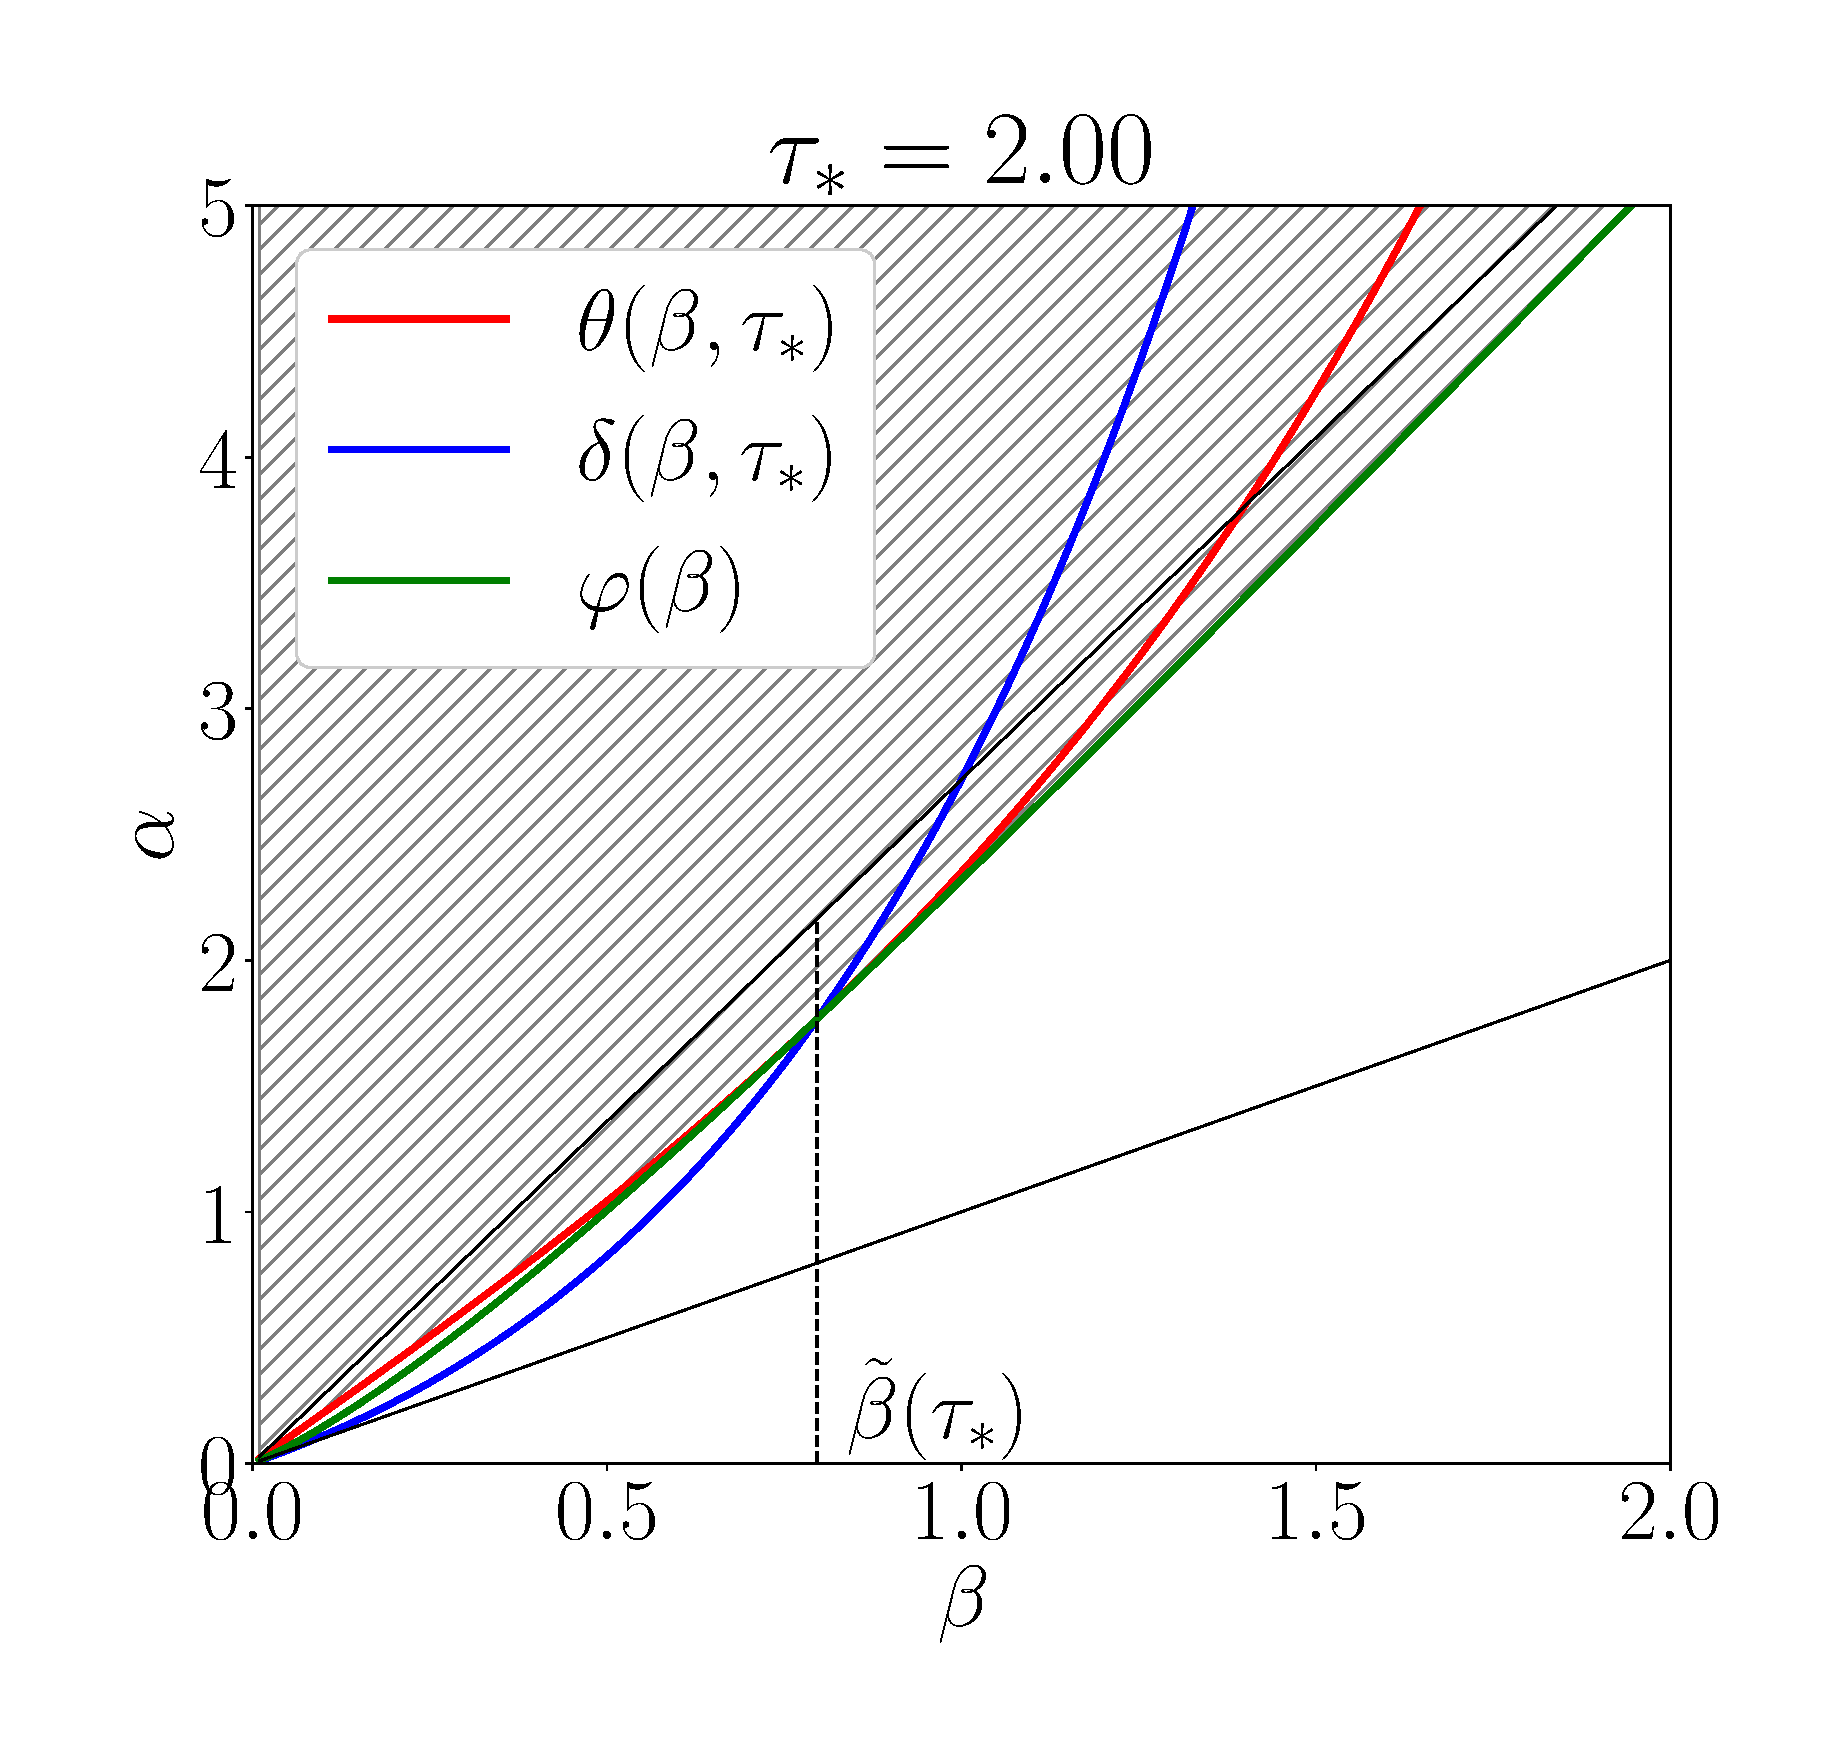
\includegraphics[width=\linewidth]{images/conditions_tau_2p00.eps}
	\end{minipage}
	\caption{Иллюстрация области параметров \eqref{eq:phi_theta_cond} при различных значениях $\tau_*$. Помимо функций $\theta$, $\varphi$ и $\delta$, на рисунках присутствуют прямые $\alpha = \beta$ и $\alpha = e\beta$.}
	\label{fig:step3_t1}
\end{figure}

Заметим, что при фиксированных $\beta$ и $\tau_*$ ограничение на $\alpha$ формулируется в виде $\alpha \geq c$ для некоторой константы $c$. Это будет важно в дальнейшем, когда мы будем искать параметры, удовлетворяющие уравнению \eqref{eq:period_equation}.


\subsection{Доказательство периодичности построенного решения}
В разделе \ref{sec:ch2/sect2/subsect_aux_result} на промежутке $[0,t_2]$ построено решение уравнения \eqref{eq:mg_relay_w} с начальной функцией из множества \eqref{eq:mg_init_set}. Показано, что оно совпадает с функцией $u_*(t)$, которая описывается формулами \eqref{eq:u_step1}, \eqref{eq:u_step2}, \eqref{eq:u_step3}, \eqref{eq:u_step4}. Для доказательства того, что получено периодическое решение с периодом $T = t_2 - t_0$, достаточно убедиться в том, что расстояние между точками $t_1$ и $t_2$ не меньше длины наибольшего запаздывания $\tau_N$. Для этого проследим за изменением функции $w(t)$ на промежутке $[t_1,t_1+\tau_N]$ и покажем, что на данном промежутке сохраняется неравенство $w(t) > 1$.

\subsection{Доказательство периодичности решения вспомогательного уравнения}

\begin{proposition}
	\label{w>1_t_1-t_1+1} Пусть выполнено \eqref{eq:cond_th_w>1_t_1+1},
	\begin{equation}
		\label{w>1_t_1+1}
		e^{\beta s_*}\left(s_*(1-e^\beta) + e^\beta \right) - 1 > 0,
	\end{equation}
	тогда функция $w(t)>1$ при $t\in (t_1, t_1 + 1]$.
\end{proposition}
\begin{proof}
	Неравенство $w(t)>1$ на промежутке $(t_1, t_1 + 1]$ с учетом $u_0 A = e^{\beta t_0}$ эквивалентно неравенству $u_0Ae^{-\beta t}(1+\alpha e^{\beta }(t-t_0-1)) >1$ или $1+\alpha e^{\beta }(t-t_0-1) > e^{\beta (t-t_0)}$.
	Заметим, что в левой части неравенства стоит аффинная функция, в правой --- экспоненциальная (выпуклая функция). Тогда для верности утверждения на $(t_1, t_1 + 1)$ достаточно, чтобы функция $w(t)$ была больше или равна $1$ в концах соответствующего отрезка. Известно, что $w(t_1) = 1$, остается проверить $w(t_1+1) \geqslant 1$. Теперь добавим, что для верности утверждения на полуинтервале $(t_1, t_1 + 1]$ последнее условие нужно усилить строгим знаком.
	Запишем это в виде:
	$$w(t_1+1) = e^{-\beta (t_1 -t_0+ 1)}( 1+\alpha e^{\beta }(t_1-t_0) )>1 .$$
	Используя равенство $\alpha = \dfrac{e^{\beta(t_1 - t_0)}-1}{e^\beta(t_1 - t_0 -1)}$, которое следует из $w(t_1)=1$, перепишем неравенство:
	$$e^{-\beta(t_1-t_0+1)}\Big(1 + \dfrac{e^{\beta(t_1 - t_0)}-1}{e^\beta(t_1 - t_0 -1)}e^\beta(t_1 - t_0) \Big)>1.$$
	После эквивалентных преобразований получим \eqref{eq:cond_th_w>1_t_1+1}.
\end{proof}

Функция $w(t)$ изменяется в точках переключения функции $u_*(t)$, к которым прибавляются все возможные запаздывания, а именно в точках из множеств
%
\[E_*\stackrel{\text{def}}{=}\{t_0 + \tau_k\},\ E_{**}\stackrel{\text{def}}{=}\{t_0 + 1 + \tau_k\},\ E_{***}\stackrel{\text{def}}{=}\{t_1 + \tau_k\},\text{ где }k=0,1,\ldots,N,\ \tau_0=1.\]
%
Отметим, что данные множества точек могут пересекаться.

Определим функции 
$$\xi(s)\stackrel{\text{def}}{=}\alpha e^{-\beta s} s ,\quad \eta(s)\stackrel{\text{def}}{=}\frac{\alpha^2}{2} e^{-\beta( s-1)} (s-1)^2$$
\begin{lemma}
	\label{lm:lem_w_*}
	При переходе через точки из множеств $E_*$, $E_{**}$, $E_{***}$ функция $w(t)$ изменяется следующим образом:
	\begin{equation}
		\label{eq:w_*}
		w(t_0 + \tau_k+0) = w(t_0 + \tau_k-0) +  \xi(t-\tau_k-t_0),
	\end{equation}
	\begin{equation}
		\label{eq:w_**}
		w(t_0 +1+ \tau_k+0) = w(t_0 +1+ \tau_k-0) +\eta(t-\tau_k-t_0), 
	\end{equation}
	\begin{equation}
		\label{eq:w_***} 
		w(t_1 + \tau_k+0) = w(t_1 + \tau_k-0)-\xi(t-\tau_k-t_0)-\eta(t-\tau_k-t_0)+
		(u_1 e^{\beta t_1}-u_0)e^{-\beta(t-\tau_k)}.
	\end{equation}
	Причём, если точка переключения принадлежит нескольким множествам, то применяются несколько  соответствующих формул одновременно.
\end{lemma}

\begin{proof}
	
	Рассмотрим переход через точку из множества $E_*$. В точке $t_0 + \tau_k$ слагаемое $u(t - \tau_k)$ изменяет форму с \eqref{eq:u_step1} %$u(t-h) = u_0e^{-\beta( t - h)}$ 
	на \eqref{eq:u_step2}. %$u(t-h) = u_0 e^{-\beta( t-h)}(\alpha A(t-h - t_0)+1)$.
	Следовательно, функция $w(t)$ при переходе через $t_0 + \tau_k$ изменяется на разность:
	% 
	\[u_0 e^{-\beta( t-\tau_k)}(\alpha A(t - \tau_k - t_0)+1) - u_0e^{-\beta( t - \tau_k)}= \alpha e^{-\beta( t-\tau_k-t_0)}(t-\tau_k-t_0).\]
	%, что указано в выражении \eqref{w_*} Леммы \ref{lem_w_*}. 
	%
	% Можно и расписать подробно
	Аналогично доказываются формулы \eqref{eq:w_**} и \eqref{eq:w_***}. При рассмотрении точек из множеств $E_{**}$ и $E_{***}$ происходит изменение аналитической формы одного из слагаемых с \eqref{eq:u_step2} на \eqref{eq:u_step3} и с \eqref{eq:u_step3} на \eqref{eq:u_step4} соответственно.
	
	Отдельно разберем ситуацию, когда некоторые из точек множеств $E_*$, $E_{**}$ и $E_{***}$ совпали. Заметим, что точки внутри множеств совпадать не могут, так как все запаздывания различны. Так же не могут совпадать точки из разных множеств с прибавлением одинакового запаздывания, так как точки $t_0$, $t_0 + 1$ и $t_1$ различны. Тогда совпасть могут только точки из разных множеств  с прибавлением разных запаздываний. Следовательно, изменение функции $w(t)$ в совпадающих точках будут происходить за счет разных слагаемых $u(t-\tau_k)$, а значит, независимо друг от друга. Тогда общее изменение функции $w(t)$ будет складываться из суммы изменений вида \eqref{eq:w_*}, \eqref{eq:w_**} и \eqref{eq:w_***}.
\end{proof}


Отметим, что добавки в формулах \eqref{eq:w_*}, \eqref{eq:w_**} неотрицательны и обращаются в ноль в соответствующих точках переключения.

\begin{lemma}
	\label{lm:lem_w>1}
	Пусть выполнены условия лемм \ref{lm:t1_existence}, \ref{lm:t1_locate} и пусть, кроме того,
	параметры удовлетворяют ограничениям \eqref{eq:cond_th_w>1_t_1+1}, \eqref{eq:cond_hair_hair_01}, \eqref{eq:cond_hair_hair_02}, \eqref{eq:cond_hair_hair_1}.
	Тогда $w(t)>1$ при $t\in(t_1,t_1+\tau_N]$.
\end{lemma}

Идея доказательства состоит в следующем. На каждом из промежутков $(t_1, t_1+\tau_k]$ мы определим функцию $\tilde{v}(t) < w(t)$ и покажем, что $1 < \tilde{v}(t)$. Тем самым, утверждение леммы \ref{lm:lem_w>1} окажется доказано.

Будем последовательно рассматривать промежутки $(t_1,t_1+1]$, $(t_1+\tau_{k-1},t_1+\tau_k]$, $k = 1,\ldots,N$. Доказывая на каждом шаге, что на соответствующем промежутке верно $w(t) > 1$, мы также доказываем, что на нём не появится новых точек переключения. Поэтому нам не потребуется рассматривать изменения функции $w(t)$, отличные от тех, что описаны в лемме \ref{lm:lem_w_*}.

Рассмотрим вспомогательную функцию $\tilde{u}(t)$, определенную на отрезке $[0,t_2]$ следующим образом (см. рис. \ref{fig:u_hair}): 
\begin{equation}
	\label{eq:u_hair}
	\tilde{u}(t)\stackrel{\text{def}}{=}\left\lbrace\begin{array}{cl}
		u_0e^{-\beta t} & \text{ при } t\in[0,t_1],
		\\
		u_1e^{-\beta (t-t_1)} & \text{ при } t\in(t_1,t_1+1+\tau_N].
	\end{array}\right.
\end{equation}
%
%%% ГРАФИК U-КУДРЯВОЕ
\begin{figure}
	\centering
	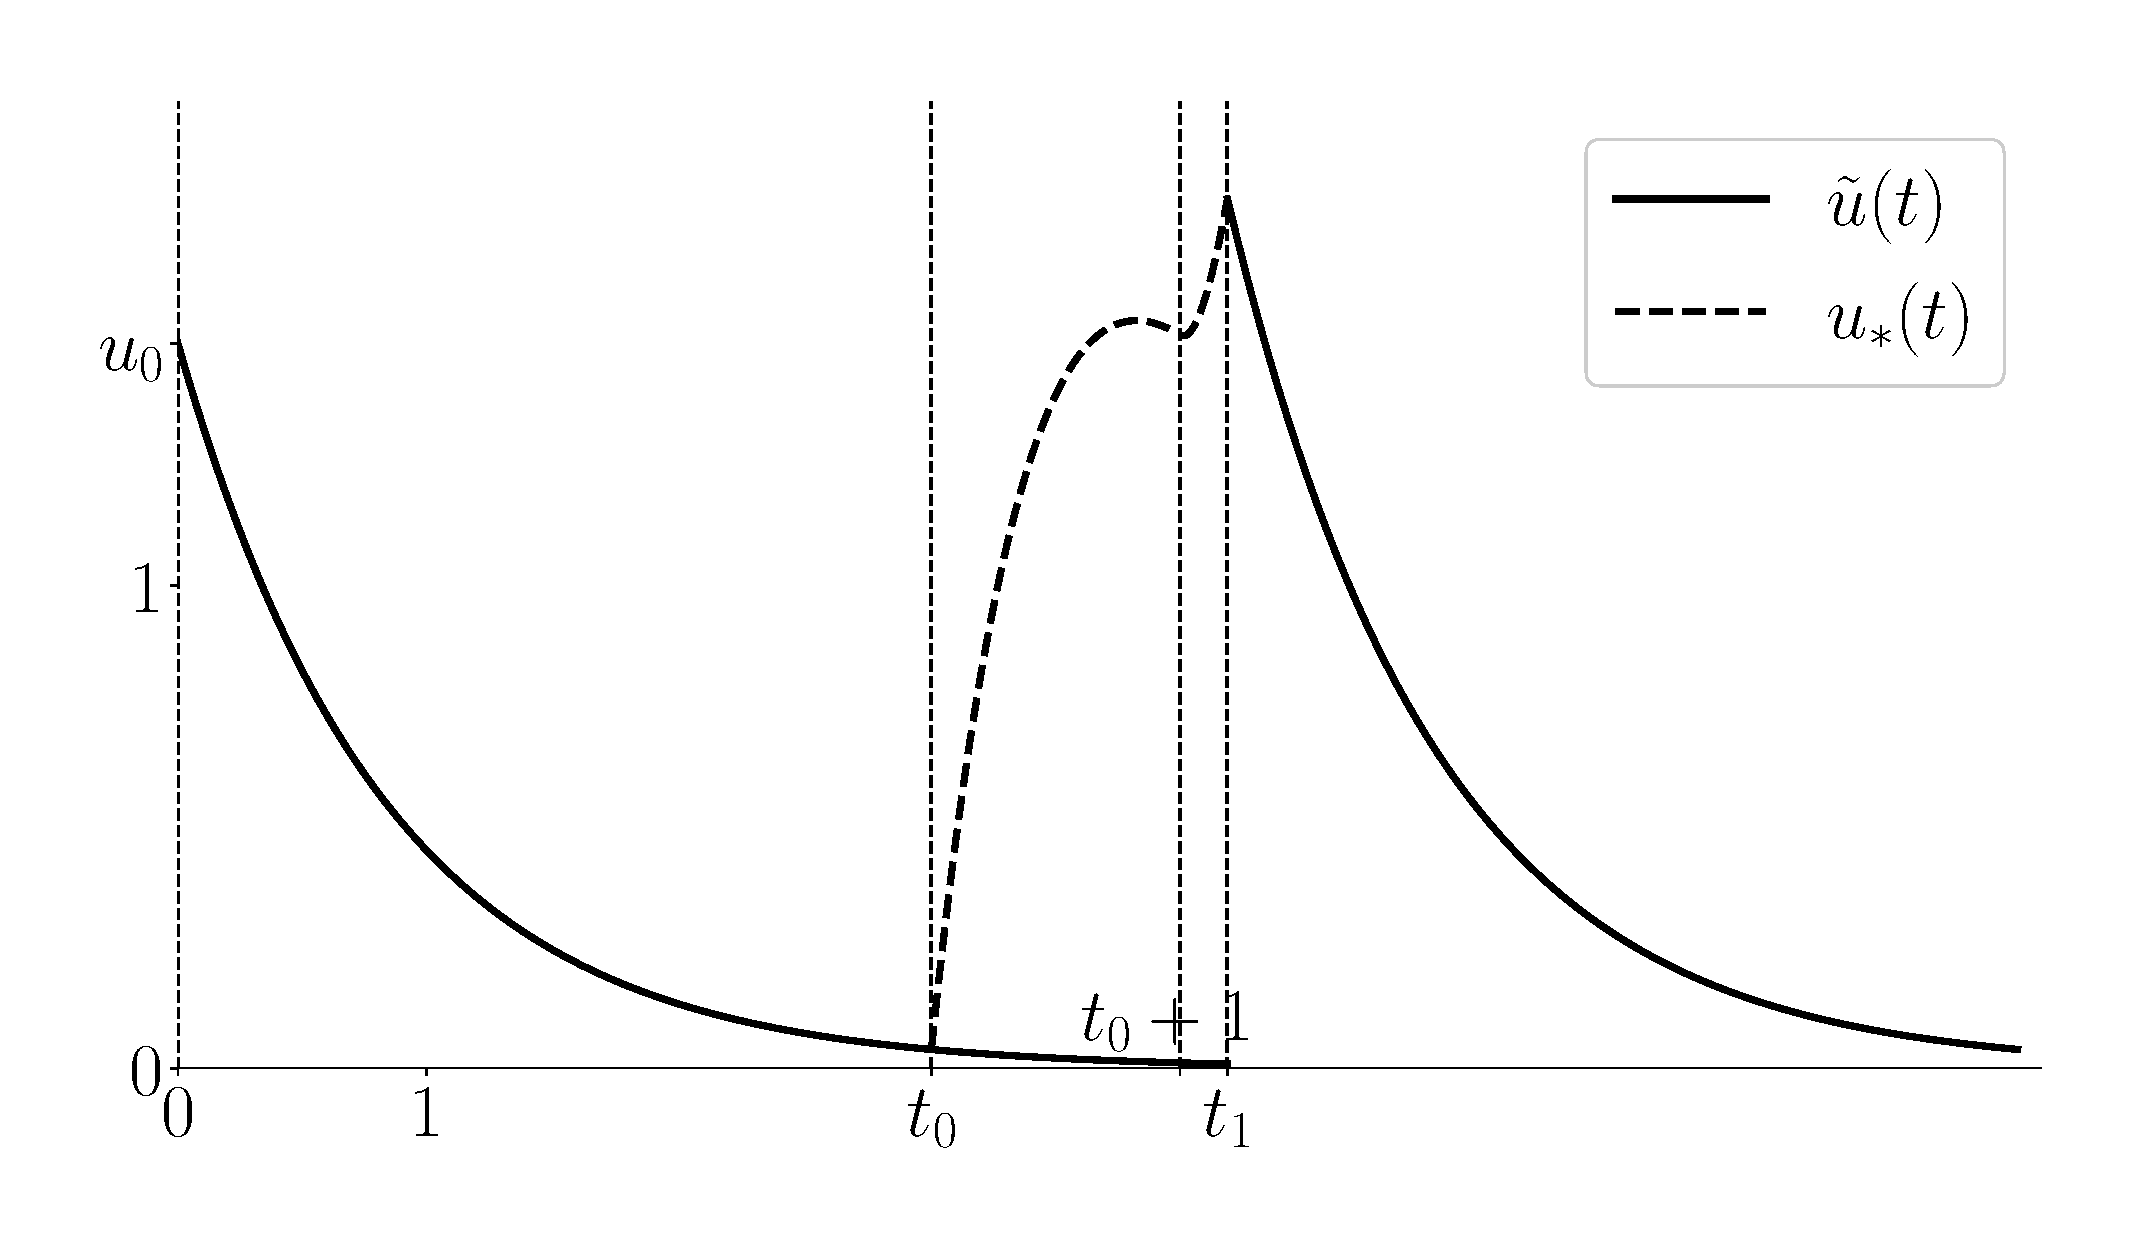
\includegraphics[width=0.7\textwidth]{u_hair.eps}
	\caption{Схематичный график функции $\tilde{u}(t)$}
	\label{fig:u_hair}
\end{figure}
%

По функции $\tilde{u}(t)$ построим функцию
%
\[
\tilde{w}(t) = \sum_{i=0}^{N}\tilde{u}(t-\tau_i),
\]
%
определенную на отрезке $[\tau_N, t_1 + \tau_N]$. Ее явный аналитический вид:
%
\begin{equation}
	\label{eq:w_hair}
	\tilde{w}(t)=
	\begin{cases}
		e^{-\beta (t-t_0)} & \text{ при } t\in[\tau_N,t_1+1],\\
		C_k e^{-\beta(t-t_0)} & \text{ при } t\in(t_1 + \tau_{k-1}, t_1 + \tau_k],\ k=1,\ldots,N,
	\end{cases}
\end{equation}
где
\[C_k = 1+\left(\frac{\alpha^2}{2}e^\beta\big( s_*-1)^2+\alpha s_*\right)\sum_{i=0}^{k-1}e^{\beta \tau_i}.\]

Функция $\tilde{w}(t)$ обладает скачками в точках %$t_1 + \tau_k$ 
множества $E_{***}$:
\begin{equation}
	\label{eq:w_hair_***} 
	\tilde{w}(t_1 + \tau_k+0) = \tilde{w}(t_1 + \tau_k-0)+
	e^{-\beta(t-\tau_k)}(u_1 e^{\beta t_1}-u_0).
\end{equation}
%
Изменение \eqref{eq:w_hair_***} функции $\tilde{w}(t)$ --- это \eqref{eq:w_***} без участия слагаемых-добавок из \eqref{eq:w_*} и \eqref{eq:w_**}. В отличие от $w(t)$, функция $\tilde{w}(t)$ не меняет форму при переходе через точки из множеств $E_*$ и $E_{**}$. Заметим также, что функция $\tilde{w}(t)$ будет разрывной в точках из $E_{***}$. Схематичный график функции $\tilde{w}(t)$ изображен на рисунке \ref{fig:w_hair}.

Теперь к этой функции <<добавим>> на отрезках $[t_0+1,t_1+1]$, $[t_0+\tau_k, t_1+\tau_k]\cap[t_1+\tau_{k-1},t_1+\tau_k]$, $k=1,\ldots,N$, слагаемые из \eqref{eq:w_*}.

Пусть
%
\[
\tilde{\xi}(s) = 
\begin{cases}
	\xi(s) & \text{ при } s\in[0,s_*],\\
	0 & \text{ при } s\notin[0,s_*].
\end{cases}
\]
%
Определим функцию $\tilde{v}(t)$ на отрезке $[\tau_N,t_1+1+\tau_N]$ следующим образом (см. рис. \ref{fig:w_hair}):
%
\[
\tilde{v}(t) =
\begin{cases}
	\tilde{w}(t)+\tilde{\xi}(t-t_0-1)& \text{ при } t\in[\tau_{N}, t_1 + 1],\\
	\tilde{w}(t)+\tilde{\xi}(t-t_0-\tau_k)& \text{ при } t\in(t_1 + \tau_{k-1}, t_1 + \tau_k],\
\end{cases}
\]
%
%
%%% ГРАФИК W-КУДРЯВОЕ и V-КУДРЯВОЕ
\begin{figure}
	\centering
	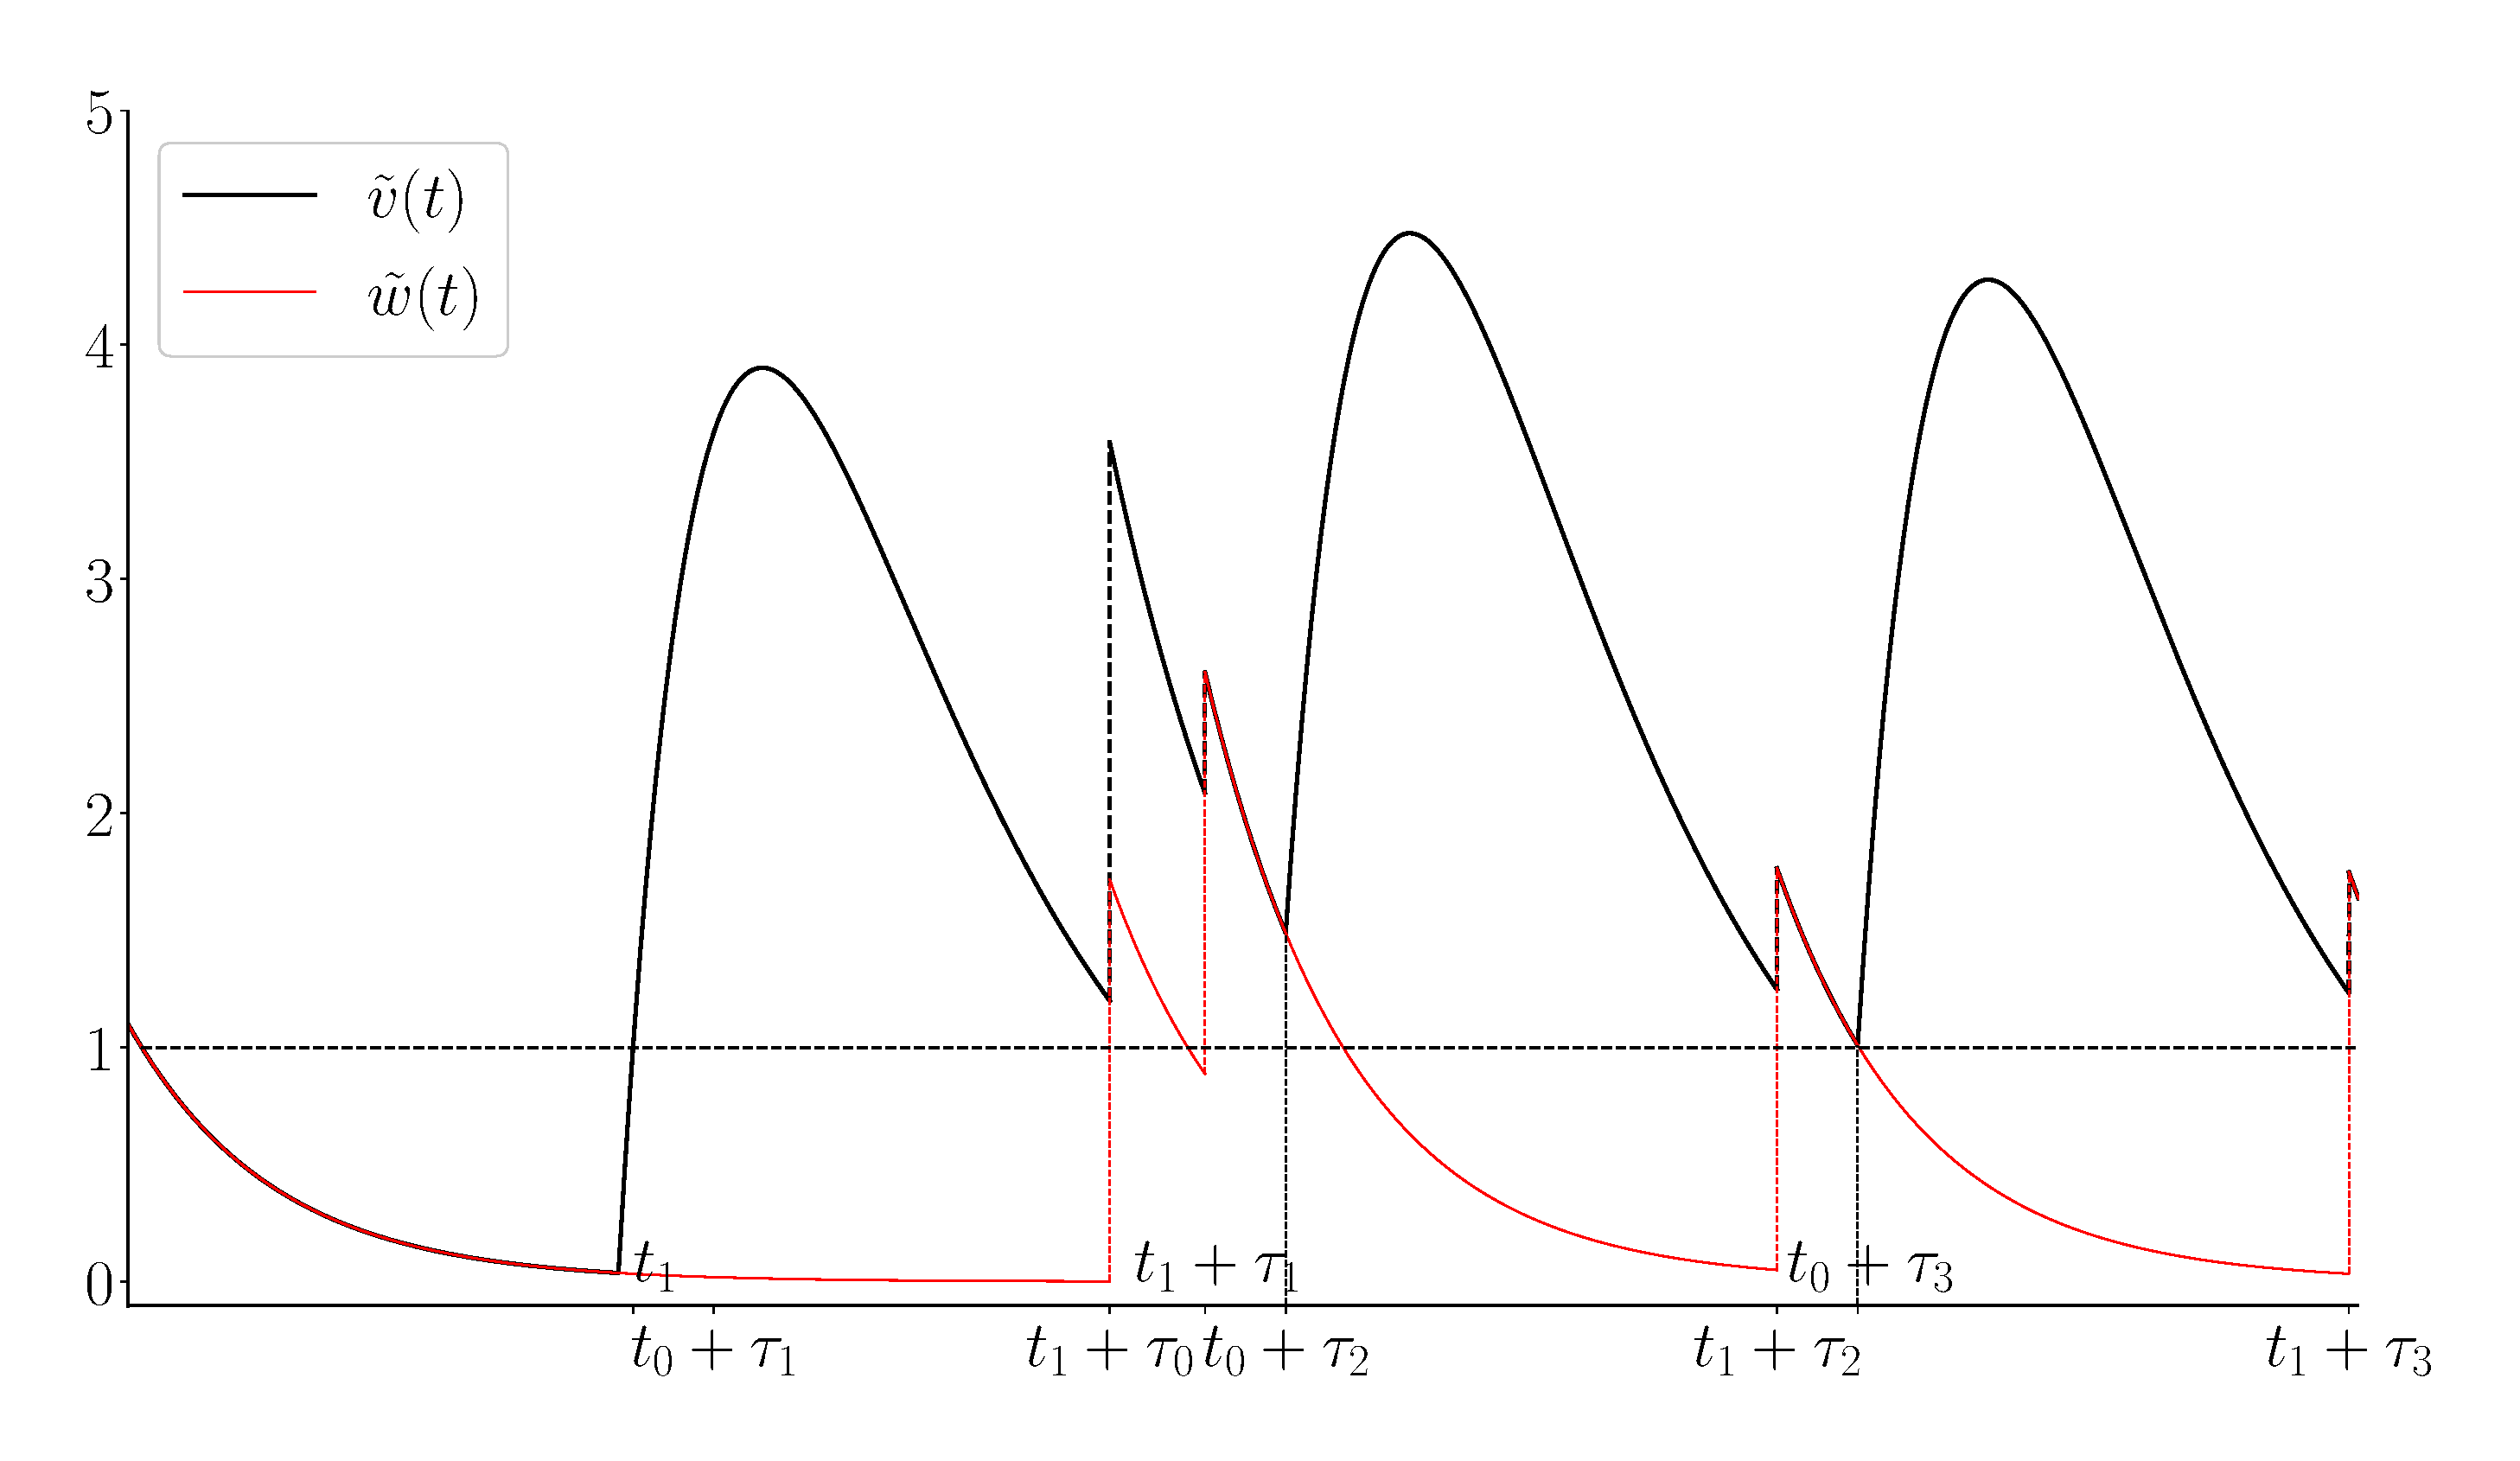
\includegraphics[width=0.7\textwidth]{w_hair.eps}
	\caption{Схематичный график функций $\tilde{w}(t)$ и $\tilde{v}(t)$. На этом рисунке $t_0+\tau_1 \notin[t_1+\tau_0,t_1+\tau_1]$, поэтому при $t\in(t_1+\tau_0,t_1+\tau_1]$ функция  $\tilde{v}(t)$ описывается формулой \eqref{eq:v_hair1} при $k=1$, и соответствующие условия того, что здесь $\tilde{v}(t)>1$, --- это формулы \eqref{eq:cond_hair_hair_02} и \eqref{eq:cond_hair_hair_1} при $k=1$. На следующем отрезке $[t_1+\tau_1,t_1+\tau_2]$ другая ситуация,  $t_0+\tau_2\in[t_1+\tau_1,t_1+\tau_2]$, поэтому здесь $\tilde{v}(t)$ описывается формулой \eqref{eq:v_hair2} при $k=2$, а соответствующие условия для $\tilde{v}(t)>1$ здесь --- это \eqref{eq:cond_hair_hair_01} и \eqref{eq:cond_hair_hair_1} при $k=2$. }
	\label{fig:w_hair}
\end{figure}
%

%
\begin{proposition}
	\label{prop:w_w_hair}
	$\tilde{w}(t)\leqslant\tilde{v}(t)\leqslant w(t)$ при $t\in[\tau_N,t_1+\tau_k]$.
\end{proposition}
\begin{proof}
	Функции $\tilde{w}(t)$ и $\tilde{v}(t)$ отличаются на неотрицательные добавки \eqref{eq:w_*}, функции $\tilde{v}(t)$ и $w(t)$ отличаются по крайней мере на неотрицательные добавки \eqref{eq:w_**}.
\end{proof}

\begin{proposition}
	\label{prop:v_hair>1}
	Пусть выполнены условия лемм \ref{lm:t1_existence}, \ref{lm:t1_locate} и ограничения \eqref{eq:cond_th_w>1_t_1+1}, \eqref{eq:cond_hair_hair_01}, \eqref{eq:cond_hair_hair_02}, \eqref{eq:cond_hair_hair_1}. Тогда 
	$\tilde{v}(t)>1$ при $t\in(t_1,\ t_1+\tau_N]$.
\end{proposition}

\begin{proof}
	Опишем $\tilde{v}(t)$ в явном виде.
	%
	\[
	\tilde{v}(t) = 
	\begin{cases}
		e^{-\beta(t-t_0)} & \text{ при } t\in[\tau_N,t_0+1],\\
		e^{-\beta(t-t_0)}+\alpha e^{-\beta (t-t_0-1)} (t-t_0-1) & \text{ при } t\in(t_0+1,t_1+1].
	\end{cases}
	\]
	%
	В зависимости от упорядоченности пары точек $t_0+\tau_k$ и $t_1+\tau_{k-1}$ возможны два варианта аналитического описания функции $\tilde{v}(t)$ на отрезке $[t_1+\tau_{k-1},t_1+\tau_k]$:
	1) если $t_0+\tau_k\in[t_1+\tau_{k-1},t_1+\tau_k]$, то
	\begin{equation}
		\label{eq:v_hair1}
		\tilde{v}(t)=
		\begin{cases}
			C_k e^{-\beta(t-t_0)} & \text{ при } t\in(t_1+\tau_{k-1},t_0+\tau_k],\\
			C_k e^{-\beta(t-t_0)} + \alpha e^{-\beta (t-t_0-\tau_k)} (t-t_0-\tau_k) & \text{ при } t\in(t_0+\tau_k,t_1+\tau_k];
		\end{cases}
	\end{equation}
		
	2) если $t_0+\tau_{k} < t_1+\tau_{k-1}$, то
	\begin{equation}
		\label{eq:v_hair2} 
		\tilde{v}(t)= C_k e^{-\beta(t-t_0)}+\alpha e^{-\beta (t-t_0-\tau_k)} (t-t_0-\tau_k) \text{ при } t\in(t_1+\tau_{k-1},t_1+\tau_k].
	\end{equation}
	
	% Сделаем замену $t=t(s)=s+\tau_k+t_0$. %Учитывая, что $u_0A=e^{\beta t_0}$, 
	% Тогда
	% \begin{enumerate}
		%     \item[1)] если $s_*\leqslant \tau_{k}-\tau_{k-1}$, то
		%     $$\tilde{v}(t(s))=\left\lbrace\begin{array}{cl}
			% C_ke^{-\beta \tau_k}e^{-\beta s} & \text{ при } t\in[s_*+\tau_{k-1}-\tau_k,0],
			% \\
			% e^{-\beta s}(\alpha s+C_ke^{-\beta \tau_k}) & \text{ при } t\in(0,s_*];
			% \end{array}\right.$$
		%     \item[2)] если $s_*>\tau_{k}-\tau_{k-1}$, то
		%     $$\tilde{v}(t(s))=e^{-\beta s}(\alpha s+C_ke^{-\beta \tau_k})  \text{ при } t\in(s_*+\tau_{k-1}-\tau_k,s_*].$$
		% \end{enumerate}
	
	Функция $C_ke^{-\beta s}$ убывает по $s$.
	
	Функция $C_ke^{-\beta \tau_k}e^{-\beta s}+\alpha e^{-\beta s} s$ обладает локальным максимумом в точке $\frac{\alpha-\beta C_ke^{-\beta \tau_k}}{\alpha \beta}$.
	%
	%Функция $e^{-\beta s}(\frac{\alpha^2}{2}e^\beta\big( s_*-1)^2+\alpha s_*+C_k)$ либо монотонно убывает, либо имеет локальные минимум и максимум. В последнем случае точка минимума оказывается меньше 1.
	%
	Тогда на любом конечном промежутке она либо монотонна, либо имеет локальный максимум, то есть достаточно проверять неравенство в концах промежутка. Это означает, что для верности неравенства $\tilde{v}(t)>1$ при $t\in(t_1,t_1+1]$ и  $t\in(t_1+\tau_{k-1},t_1+\tau_k]$, $k = 1,\ldots,N$,  достаточно, чтобы выполнялось  
	\begin{equation}
		\label{eq:cond_v_hair>1_1}
		e^{-\beta(t-t_0)}+\alpha e^{-\beta (t-t_0-1)} (t-t_0-1)|_{t=t_1}\geqslant 1,
	\end{equation}
	\begin{equation}
		\label{eq:cond_v_hair>1_2}
		e^{-\beta(t-t_0)}+\alpha e^{-\beta (t-t_0-1)} (t-t_0-1)|_{t=t_1+1}>1,
	\end{equation}
	\begin{equation}
		\label{eq:cond_v_hair>1_3}
		C_k e^{-\beta(t-t_0)}+\alpha e^{-\beta (t-t_0-\tau_k)} (t-t_0-\tau_k)|_{t=\max\{t_0+\tau_k,t_1+\tau_{k-1}\}}>1,
	\end{equation}
	\begin{equation}
		\label{eq:cond_v_hair>1_4}
		C_k e^{-\beta(t-t_0)}+\alpha e^{-\beta (t-t_0-\tau_k)} (t-t_0-\tau_k)|_{t=t_1+\tau_k}>1.
	\end{equation}
	Неравенство \eqref{eq:cond_v_hair>1_1} справедливо и обращается в равенство, поскольку $s_*=t_1-t_0$ --- это корень уравнения $e^{\beta s}-1=\alpha e^{\beta}(s-1)$. Неравенство \eqref{eq:cond_v_hair>1_2} эквивалентно \eqref{eq:cond_th_w>1_t_1+1}. Неравенство \eqref{eq:cond_v_hair>1_3} при $t_0+\tau_k\geqslant t_1+\tau_{k-1}$ обращается в \eqref{eq:cond_hair_hair_01}. При при $t_0+\tau_k<t_1+\tau_{k-1}$ это неравенство заменим более сильным
	\[C_ke^{-\beta(t-t_0)}|_{t=t_1+\tau_{k-1}}>1,\]
	которое эквивалентно \eqref{eq:cond_hair_hair_02}.
	Неравенство \eqref{eq:cond_v_hair>1_4} эквивалентно \eqref{eq:cond_hair_hair_1}.
	
	% Отметим, что неравенство (\ref{cond_hair_hair_02}) при $k=1$ заменяется более слабым, но достаточным неравенством (\ref{cond_th_w>1_t_1+1}), гарантирующим, что 
	% \begin{figure}
		%     \centering
		%     \includegraphics[width=0.7\textwidth]{w_hair_k.png}
		%     \caption{Схематичный график функции $\tilde{w}_k(t)$}
		%     \label{pic:w_hair}
		% \end{figure}
\end{proof}

Справедливость леммы \ref{lm:lem_w>1} следует из утверждений \ref{prop:w_w_hair} и \ref{prop:v_hair>1}.

\section{Дискретные бегущие волны}\label{sec:ch2/sect3}

Докажем, что при фиксированных параметрах $\alpha, \beta$ и некотором $\Delta$ существует периодическое решение системы \eqref{eq:mg_relay_1} с периодом $T(\Delta)$, удовлетворяющее уравнению \eqref{eq:period_equation} при $p = 1$.

Пусть $\Delta > 1$, тогда запаздывания равны $\{1, \Delta, 2\Delta, \ldots, N\Delta\}$. В этом случае нормировка \eqref{eq:mg_norm} не изменяет уравнение периодов \eqref{eq:period_equation}.  Подставим значение $T(\Delta)$ из \eqref{eq:mg_period_T} в \eqref{eq:period_equation} при $p = 1$:
%
\begin{equation}
	\label{eq:period_eq}
	\dfrac{1}{\beta}\ln\left( \frac{\alpha^2}{2}Ae^{\beta}( s_*-1)^2+\alpha A s_* + 1\right) = \Delta (N + 1).
\end{equation}
%
Элементарными преобразованиями сводим уравнение к виду:
\begin{equation}
	\label{eq:period_eq_exp}
	\dfrac{1}{A}\left(e^{\beta\Delta(N + 1)} - 1\right) = \dfrac{\alpha^2}{2}e^{\beta}( s_* - 1)^2 + \alpha s_*.
\end{equation}

\begin{proposition}
	$\lim\limits_{\alpha\to+\infty} s_*(\alpha) = 1 + 0$.
\end{proposition}
\begin{proof}
	Значение $s_*$ находится как меньший корень уравнения $\alpha = \theta(\beta, s_*)$. В утверждении \ref{prop:phi_theta} было показано, что при фиксированном $\beta$ у функции $\theta(\beta,  s_*)$ ровно одна точка минимума $ s_*^{\text{min}}$ (см. рисунок \ref{fig:theta_func_min}), при этом
	%
	\begin{equation}
		\lim\limits_{s_* \to 1+0} \theta(\beta, s_*) = \lim\limits_{s_*\to +\infty} \theta(\beta,  s_*) = +\infty.
	\end{equation}
	%
	Тогда у функции $s_*(\alpha)$ две непрерывных ветви $s_* \in (1;  s_*^{\text{min}}]$ и $ s_* \in [ s_*^{\text{min}}; +\infty)$. Меньший корень лежит на левой ветви, но тогда $\lim\limits_{\alpha\to+\infty} s_*(\alpha)= 1 + 0$.
\end{proof}
%
%%% ФУНКЦИЯ THETA
\begin{figure}
	\centering
	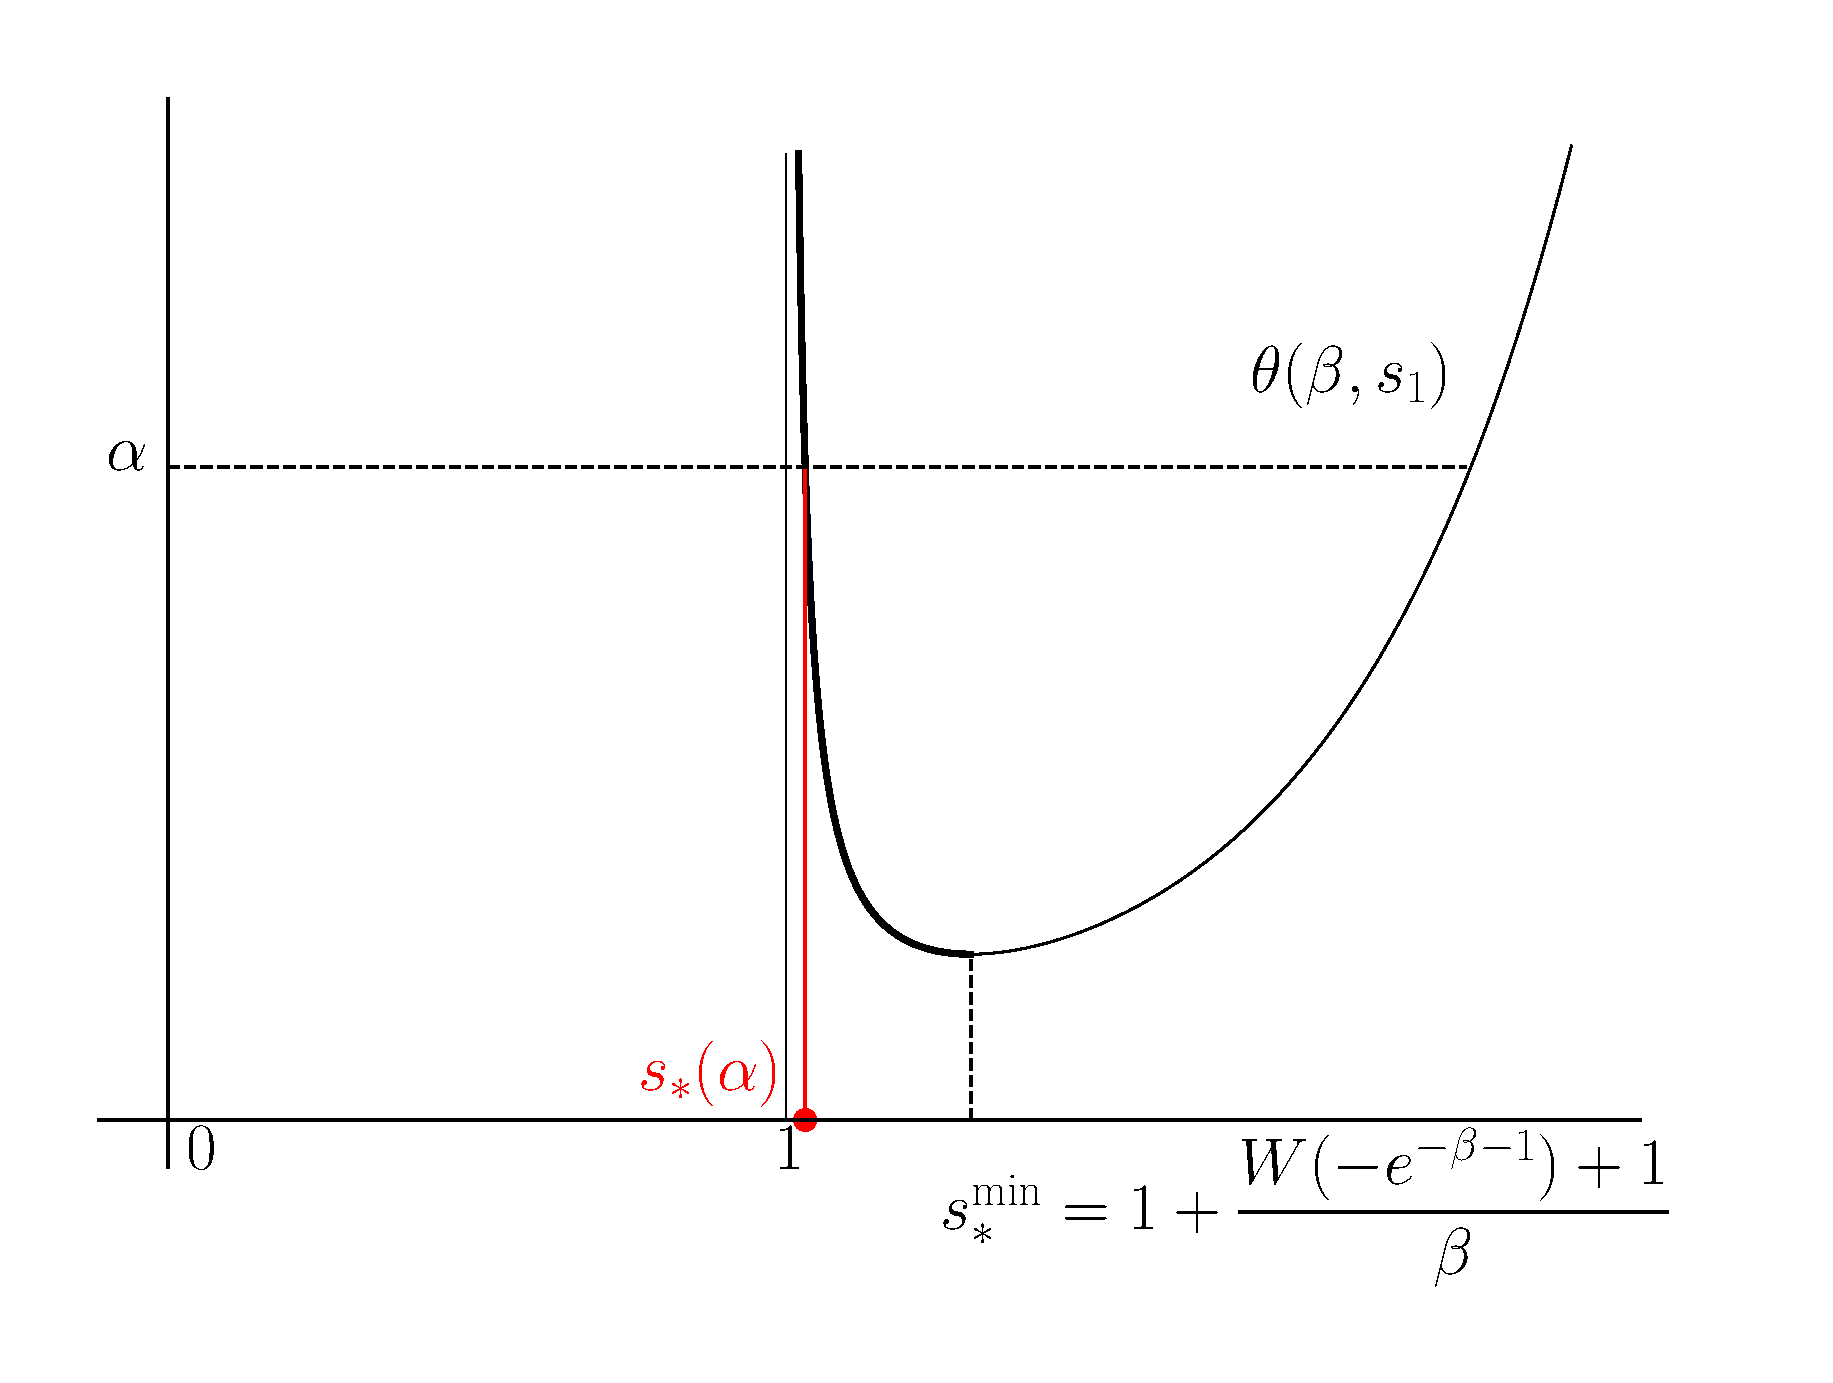
\includegraphics[width=0.7\textwidth]{theta.eps}
	\caption{При фиксированном $\beta$ функция $\theta(\beta,  s_*)$ имеет одну точку минимума $ s_*^{\min}$ и два промежутка монотонности $(1; + s_*^{\min}]$ и $[ s_*^{\min}; +\infty)$. Значение $ s_*(\alpha)$ определяется как меньший корень уравнения $\alpha = \theta(\beta,  s_*)$, поэтому левая ветвь (выделена толстой линией) определяет зависимость $ s_*(\alpha)$.}
	\label{fig:theta_func_min}
\end{figure}


%
\begin{proposition}
	Правая часть уравнения \eqref{eq:period_eq_exp} стремится к $+\infty$ при $\alpha \to +\infty$.
\end{proposition}
\begin{proof}
	Заменим в правой части уравнения \eqref{eq:period_eq_exp} $\alpha = \dfrac{e^{\beta s_*} - 1}{e^{\beta}(s_* - 1)}$:
	\begin{equation}
		\dfrac{\alpha^2}{2}e^{\beta}( s_* - 1)^2 + \alpha s_* = \dfrac{1}{2}e^{-\beta}(e^{\beta s_*} - 1)^2 + \dfrac{s_*}{s_* - 1}\dfrac{e^{\beta s_*} - 1}{e^{\beta}}.
	\end{equation}
	Устремим $\alpha \to +\infty$, тогда $s_* \to 1 + 0$ и выражение стремится к $+\infty$ за счёт множителя $\dfrac{s_*}{s_* - 1} > 0$.
\end{proof}

Получаем, что левая часть уравнения \eqref{eq:period_eq_exp} от $\alpha$ не зависит, а правая принимает сколь угодно большие значения при больших $\alpha$.

В свою очередь, правая часть не зависит от $\Delta$, а левая эквивалентна $e^{\beta\Delta}$ при $\Delta \to +\infty$:
$$
\dfrac{1}{A(\Delta)}\left(e^{\beta\Delta(N + 1)} - 1\right) = \dfrac{e^{\beta\Delta(N + 1)} - 1}{e^{\beta} - 1 + \frac{e^{\beta\Delta(N + 1)} - 1}{e^{\beta\Delta} - 1}} \sim e^{\beta \Delta}.
$$

Таким образом, при фиксированных $\alpha$ и $\beta$ мы можем добиться равенства в уравнении \eqref{eq:period_eq_exp} за счёт увеличения $\Delta$; для этого нам нужно, чтобы сова нашла хвост и левая часть уравнения была меньше правой для некоторого $\Delta$.

Фиксируем параметр $\beta > 0$.

Рассмотрим условие \eqref{eq:cond_th_w>1_t_1+1}. Произведём замену $\alpha = \dfrac{e^{\beta s_*} - 1}{e^{\beta}(s_* - 1)}$. Получим: 
\begin{equation}
	e^{-\beta  s_*} \left(e^{-\beta} + \frac{e^{\beta s_*} - 1}{e^{\beta}(s_* - 1)}s_*\right) > 1.
\end{equation}
%

\begin{proposition}
	Функция 
	\begin{equation}
		h(s_*) = e^{-\beta  s_*} \left(e^{-\beta} + \frac{e^{\beta s_*} - 1}{e^{\beta}(s_* - 1)}s_*\right)
	\end{equation}
	убывает при $s_* \geqslant 1$.
\end{proposition}
%
\begin{proof}
	\begin{equation}
		\dfrac{d}{ds_*}h(s_*) = -\dfrac{e^{-\beta(s_* + 1)} (e^{\beta s_*} - \beta s_* - 1 + \beta)}{(s_* - 1)^2}.
	\end{equation}
	% Из разложения экспоненты
	Поскольку $e^{\beta s_*} > 1 + \beta s_*$, получаем, что $\dfrac{d}{ds_*}h(s_*) < 0$, следовательно, $h$ убывает.
\end{proof}

Это значит, что если значение $s_* =  s_*^0 > 1$ удовлетворяет условию \eqref{eq:cond_th_w>1_t_1+1}, то значения $1 \leqslant  s_* \leqslant s_*^0$ также ему удовлетворяют.

Пусть $s_* = 1 + \dfrac{1}{e^{\beta}}$, тогда
\begin{equation}
	\alpha = \frac{e^{\beta s_*} - 1}{e^{\beta}(s_* - 1)} = e^{\beta(1 + e^{-\beta})} - 1.
\end{equation}

Убедимся, что выполнено условие \eqref{eq:cond_th_w>1_t_1+1}:
\begin{multline}
	e^{-\beta s_*}(e^{-\beta} + \alpha s_*) =
	e^{-\beta (1 + e^{-\beta})}\left(e^{-\beta} + (1 + e^{-\beta})(e^{\beta(1 + e^{-\beta})} - 1)\right) =\\
	= e^{-\beta (1 + e^{-\beta})} e^{-\beta} + (1 + e^{-\beta}) - (1 + e^{-\beta})e^{-\beta (1 + e^{-\beta})} = \\ = 1 + e^{-\beta} - e^{-\beta (1 + e^{-\beta})} > 1.
\end{multline}

Поскольку при увеличении $\alpha$ значение $s_*$ убывает, условие \eqref{eq:cond_th_w>1_t_1+1} будет выполнено при всех $\alpha \geqslant e^{\beta(1 + e^{-\beta})} - 1$.

Теперь нужно проверить выполнение условий Леммы \ref{lm:t1_locate}, которые соответствуют условиям \eqref{eq:cond_thm1} и \eqref{eq:cond_thm2} теоремы \ref{thm:mg_auxiliary_main}.

\begin{proposition}
	\label{prop:alpha_greater_phi}
	Если $\alpha > e^{\beta(1 + e^{-\beta})} - 1$, то $\alpha > \varphi(\beta)$.
\end{proposition}
\begin{proof}
	Согласно утверждению \ref{prop:phi_theta}, $\theta(\beta, \tau_*) \geqslant \varphi(\beta)$ независимо от выбора $\tau_*$. Положим $\tau_* = 2$ и докажем, что $e^{\beta(1 + e^{-\beta})} - 1 > \theta(\beta, 2)$.
	%
	\[
	e^{\beta(1 + e^{-\beta})} - 1 >
	e^{\beta} (1 + \beta e^{-\beta}) - 1 =
	e^{\beta} + \beta - 1 > e^{\beta} + e^{-\beta} = \theta(\beta, 2).
	\]
\end{proof}

Зафиксируем $\alpha, \beta$ и положим $\Delta =  s_*(\alpha)$. Тогда условие $\alpha \geqslant \theta(\beta, \Delta)$ выполнено (поскольку обращается в равенство).

\begin{proposition}
	При $s_* = \Delta < 1 + \frac{1}{e^{\beta}}$ верно неравенство
	$$
	\dfrac{1}{A(\Delta)}\left(e^{\beta\Delta(N + 1)} - 1\right) \leqslant \dfrac{\alpha^2}{2}e^{\beta}(s_* - 1)^2 + \alpha s_*.
	$$
\end{proposition}
\begin{proof}
	Оценим левую часть:
	\[
	\dfrac{1}{A(\Delta)}\left(e^{\beta\Delta(N + 1)} - 1\right) = \dfrac{e^{\beta\Delta(N + 1)} - 1}{e^{\beta} - 1 + \frac{e^{\beta\Delta(N + 1)} - 1}{e^{\beta\Delta} - 1}} < e^{\beta \Delta} - 1.
	\]
	%
	Докажем, что правая часть больше $e^{\beta \Delta} - 1$:
	\begin{multline*}
		\dfrac{\alpha^2}{2}e^{\beta}(\Delta - 1)^2 + \alpha\Delta = \dfrac{1}{2}e^{-\beta}(e^{\beta\Delta} - 1)^2 + \dfrac{\Delta}{\Delta - 1}\dfrac{e^{\beta\Delta} - 1}{e^{\beta}} > e^{\beta \Delta} - 1 \Leftrightarrow\\
		\dfrac{1}{2}(e^{\beta\Delta} - 1) + \dfrac{\Delta}{\Delta - 1} > e^{\beta} \Leftrightarrow
		\dfrac{1}{2}(e^{\beta\Delta} - 1) + 1 + \dfrac{1}{\Delta - 1} > e^{\beta}.
	\end{multline*}
	Поскольку $1 < \Delta < 1 + \frac{1}{e^{\beta}}$,
	$$
	\dfrac{1}{2}(e^{\beta\Delta} - 1) + 1 + \dfrac{1}{\Delta - 1} \geqslant \dfrac{1}{2}(e^{\beta\Delta} - 1) + 1 + e^{\beta} > e^{\beta},
	$$
	что и требовалось.
\end{proof}

% Вроде бы эта лемма следует из того, что gamma определяется как левый корень уравнения, а он левее точки минимума.
\begin{lemma}
	\label{lm:delta_min}
	$$\dfrac{W(-e^{-\beta - 1}) + 1}{\beta} > \dfrac{1}{e^{\beta}}.$$
\end{lemma}
\begin{proof}
	\begin{multline*}
		\dfrac{W(-e^{-\beta - 1}) + 1}{\beta} > \dfrac{1}{e^{\beta}} \Leftrightarrow
		W(-e^{-\beta - 1}) > \beta e^{-\beta} - 1 \Leftrightarrow \\
		-e^{-\beta - 1} > (\beta e^{-\beta} - 1)\exp(\beta e^{-\beta} - 1) \Leftrightarrow \\
		\exp(-\beta - \beta e^{-\beta}) < 
		1 - \beta e^{-\beta} \Leftrightarrow \exp(-\beta(1 + e^{-\beta})) < 1 - \beta e^{-\beta}.
	\end{multline*}
	Поскольку $\exp(-\beta(1 + e^{-\beta})) < e^{-\beta}$, докажем, что $e^{-\beta} < 1 - \beta e^{-\beta}$:
	\[
	e^{-\beta} < 1 - \beta e^{-\beta} \Leftrightarrow e^{\beta} > 1 + \beta,
	\]
	что верно при любом $\beta > 0$.
\end{proof}

Функция $\theta(\beta, \Delta)$ убывает на промежутке $(1; \Delta_{\text{min}}]$, где (см. утверждение \ref{prop:phi_theta})
%
\[\Delta_{\text{min}} = 1 + \dfrac{W(-e^{-\beta - 1}) + 1}{\beta} > 1 + \dfrac{1}{e^{\beta}}\]
%
по лемме \ref{lm:delta_min}, значит, условие $\alpha > \theta(\beta; \Delta)$ на нём также будет выполнено. %% на самом деле, при delta > 2 ограничение на theta стабилизируется, но так даже лучше, поэтому пофигу.

При $\Delta > \Delta_{\text{min}}$ уже требуется выполнение условия $\alpha \geqslant \varphi(\beta)$, а оно выполняется согласно утверждению \ref{prop:alpha_greater_phi}.

Таким образом, условия леммы 
\ref{lm:t1_locate} остаются верны при увеличении $\Delta$. Значит, найдётся $\Delta$, удовлетворяющее уравнению \eqref{eq:period_eq_exp}.

Докажем, что при определённых таким образом параметрах $\alpha, \beta, \Delta$ выполнены условия леммы \ref{lm:lem_w>1}, которые соответствуют условиям \eqref{eq:cond_hair_hair_01}, \eqref{eq:cond_hair_hair_02}, \eqref{eq:cond_hair_hair_1}) теоремы \ref{thm:mg_auxiliary_main}. По построению $s_* < \tau_k - \tau_{k - 1} = \Delta$, поэтому при $k \geqslant 2$ мы должны проверять набор условий \eqref{eq:cond_hair_hair_01}:
\[
\frac{\alpha^2}{2}e^\beta(s_*-1)^2+\alpha s_* > \frac{e^{\beta \tau_k}-1}{\sum_{i=0}^{k-1}e^{\beta \tau_i}},\quad k=1,\ldots,N.
\]
%
Перепишем правую часть с учётом $\Delta > 1$.
\[
\frac{e^{\beta \tau_k}-1}{\sum_{i=0}^{k-1}e^{\beta \tau_i}} = \frac{e^{\beta\Delta k } - 1}{e^{\beta} - 1 + \frac{e^{\beta\Delta k} - 1}{e^{\beta\Delta} - 1}} = \frac{1}{\frac{e^{\beta} - 1}{e^{\beta\Delta k} - 1} + \frac{1}{e^{\beta\Delta} - 1}}.
\]
%
Заметим, что это выражение возрастает по $k$, поэтому достаточно выполнение условия при $k = N$. Но при подстановке $k = N + 1$ мы получаем равенство \eqref{eq:period_eq_exp}, поэтому при $k \leqslant N$ оно обратится в нужное нам неравенство.

При $k = 1$ и $s_* > \tau_1 - \tau_0 = \Delta - 1$ нужно проверять условие \eqref{eq:cond_hair_hair_02}. Докажем, что оно слабее условия \eqref{eq:cond_th_w>1_t_1+1}, которое было проверено ранее. Запишем условие \eqref{eq:cond_hair_hair_02} при $k=1$:
\[
\frac{\alpha^2}{2} e^{\beta}(s_* - 1)^2 + \alpha s_* > \frac{e^{\beta (s_* + 1)} - 1}{e^{\beta}} \Leftrightarrow \left(\frac{\alpha^2}{2} e^{\beta}(s_* - 1)^2 + \alpha s_* + e^{-\beta}\right)e^{-\beta s_*} > 1.
\]
%
Но нам известно, что из условия \eqref{eq:cond_th_w>1_t_1+1},
\[
\left(\alpha s_* + e^{-\beta}\right)e^{-\beta s_*} > 1,
\]
%
а положительная добавка
\[\dfrac{\alpha^2}{2} e^{\beta}(s_* - 1)^2 e^{-\beta s_*}\]
делает неравенство ещё строже.

% На самом деле так не бывает, \Delta < 2.
Если же $s_* \leqslant \Delta - 1$, то для случая $k = 1$ верны те же рассуждения, что и для случая $2 \leqslant k \leqslant N$.

Для выполнения условий \eqref{eq:cond_hair_hair_1}:
\[
\frac{\alpha^2}{2}e^\beta(-1)^2+\alpha s_*>\frac{e^{\beta \tau_k}(e^{\beta s_*}-\alpha s_*)-1}{\sum_{i=0}^{k-1}e^{\beta \tau_i}},\quad k = 1,\ldots, N
\]
достаточно проверить, что верно неравенство
\[
e^{\beta s_*}-\alpha s_* \leqslant 1,
\]
тогда они окажутся слабее уже доказанного набора условий \eqref{eq:cond_hair_hair_01}. Замечание: мы действительно доказали их справедливость при всех $1 \leqslant k \leqslant N$, но при $k = 1$, возможно, проверяется условие из набора \eqref{eq:cond_hair_hair_02}.

Выполним замену $e^{\beta s_*} - 1 = \alpha e^\beta (s_* - 1)$.
%
\[
\alpha e^{\beta}(s_* - 1) - \alpha s_* \leqslant 0 \Leftrightarrow e^{\beta}(s_* - 1) - s_* \leqslant 0 \Leftrightarrow s_* \leqslant 1 + \frac{1}{e^{\beta} - 1}.
\]
%
По построению $s_* < 1 + \frac{1}{e^{\beta}}$, поэтому неравенство верно.
%
Из результатов, полученные в данном разделе, следует
%
\begin{theorem}
	\label{thm:relay_main}
	Для произвольных 
	%
	\begin{equation}
		\label{eq:constraints_parameters_final}
		\beta > 0, \alpha \geq e^{\beta\left(1 + \frac{1}{e^{\beta}}\right)} - 1
	\end{equation}
	%
	найдётся $\Delta > 1$, при котором набор параметров $\alpha, \beta, \Delta$ удовлетворяет уравнению \eqref{eq:period_eq} и условиям \eqref{eq:cond_thm1}, \eqref{eq:cond_thm2}, \eqref{eq:cond_th_w>1_t_1+1}, \eqref{eq:cond_hair_hair_01}, \eqref{eq:cond_hair_hair_02}, \eqref{eq:cond_hair_hair_1} теоремы \ref{thm:mg_auxiliary_main}.
\end{theorem}


\section{Результаты численного анализа системы}\label{sec:ch2/sect4}
%
Численный анализ системы, результаты которого изображены на рис. \ref{fig:periodic_solution}, показывает, что при ограничениях на параметры \eqref{eq:constraints_parameters_final} и для разных начальных условий, решение системы \eqref{eq:system_relay} стремится к режиму дискретных бегущих волн, аналитическое описание которого задаётся формулой \eqref{eq:discrete_wave}, где функция $u(t)$ описана формулами \eqref{eq:u_star}, \eqref{eq:mg_period_T}, а сдвиг $\Delta$ вычисляется из уравнения \eqref{eq:period_equation} при $p = 1$. Результаты анализа позволяют предположить глобальную устойчивость описанного предельного цикла системы.

На рисунках \ref{fig:solution_2d} и \ref{fig:solution_3d} приведены результаты численного эксперимента для систем \eqref{eq:system_relay} и \eqref{eq:mg_full_renormed}. Отметим, что при $\gamma=100$ графики решений систем \eqref{eq:system_relay} и \eqref{eq:mg_full_renormed} визуально не отличимы.

% Картинки 2022-04-30-численный-счёт.ipynb

\begin{figure}[!ht]
	\centering
	\includegraphics[width=\textwidth]{a5p0_b1p2_N2_solution_start.eps}
	\includegraphics[width=\textwidth]{a5p0_b1p2_N2_const_start.eps}
	\includegraphics[width=\textwidth]{a5p0_b1p2_N2_random_start.eps}
	\caption{Численные решения системы \eqref{eq:MG_rele} при  $\alpha = 5.0$, $\beta = 1.2$, $N = 2$ и различных начальных условиях. Слева: решение $u_0$ (чёрная линия), $u_1$ (красная линия), $u_2$ (синяя линия). Справа: псевдофазовые портреты соответствующих решений в координатах $(u_0, u_1, u_2)$.}
	\label{fig:periodic_solution}
\end{figure}

\begin{figure}
	\centering
	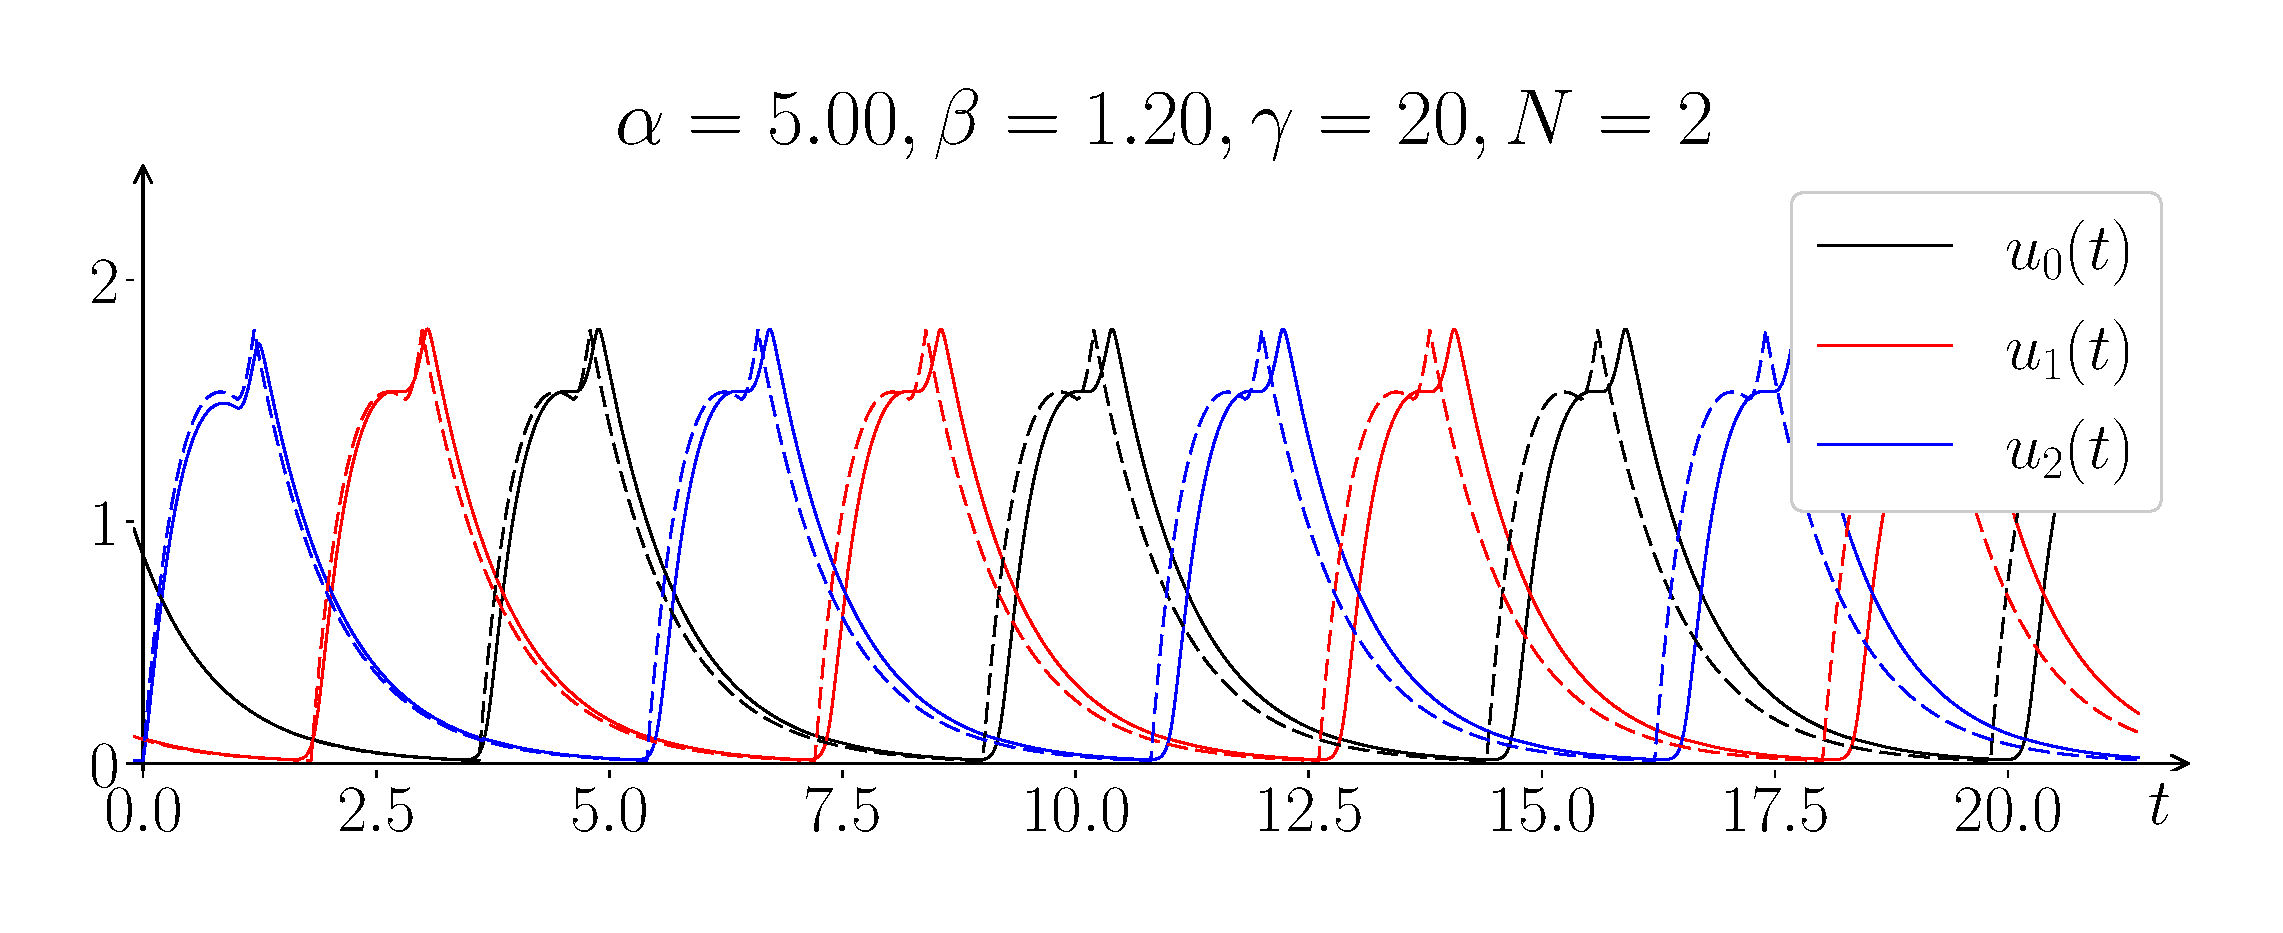
\includegraphics[width=\textwidth]{alpha_5_beta_1p2_multi.eps}
	\caption{Пунктирной линией изображено периодическое решение предельной системы  \eqref{eq:system_relay}, полученное численно при $N = 2, \alpha = 5.0, \beta = 1.2, \Delta \approx 1.801$. Сплошная линия изображает решение системы \eqref{eq:mg_full_renormed} при $\gamma = 20$.}
	\label{fig:solution_2d}
\end{figure}

\begin{figure}
	\centering
	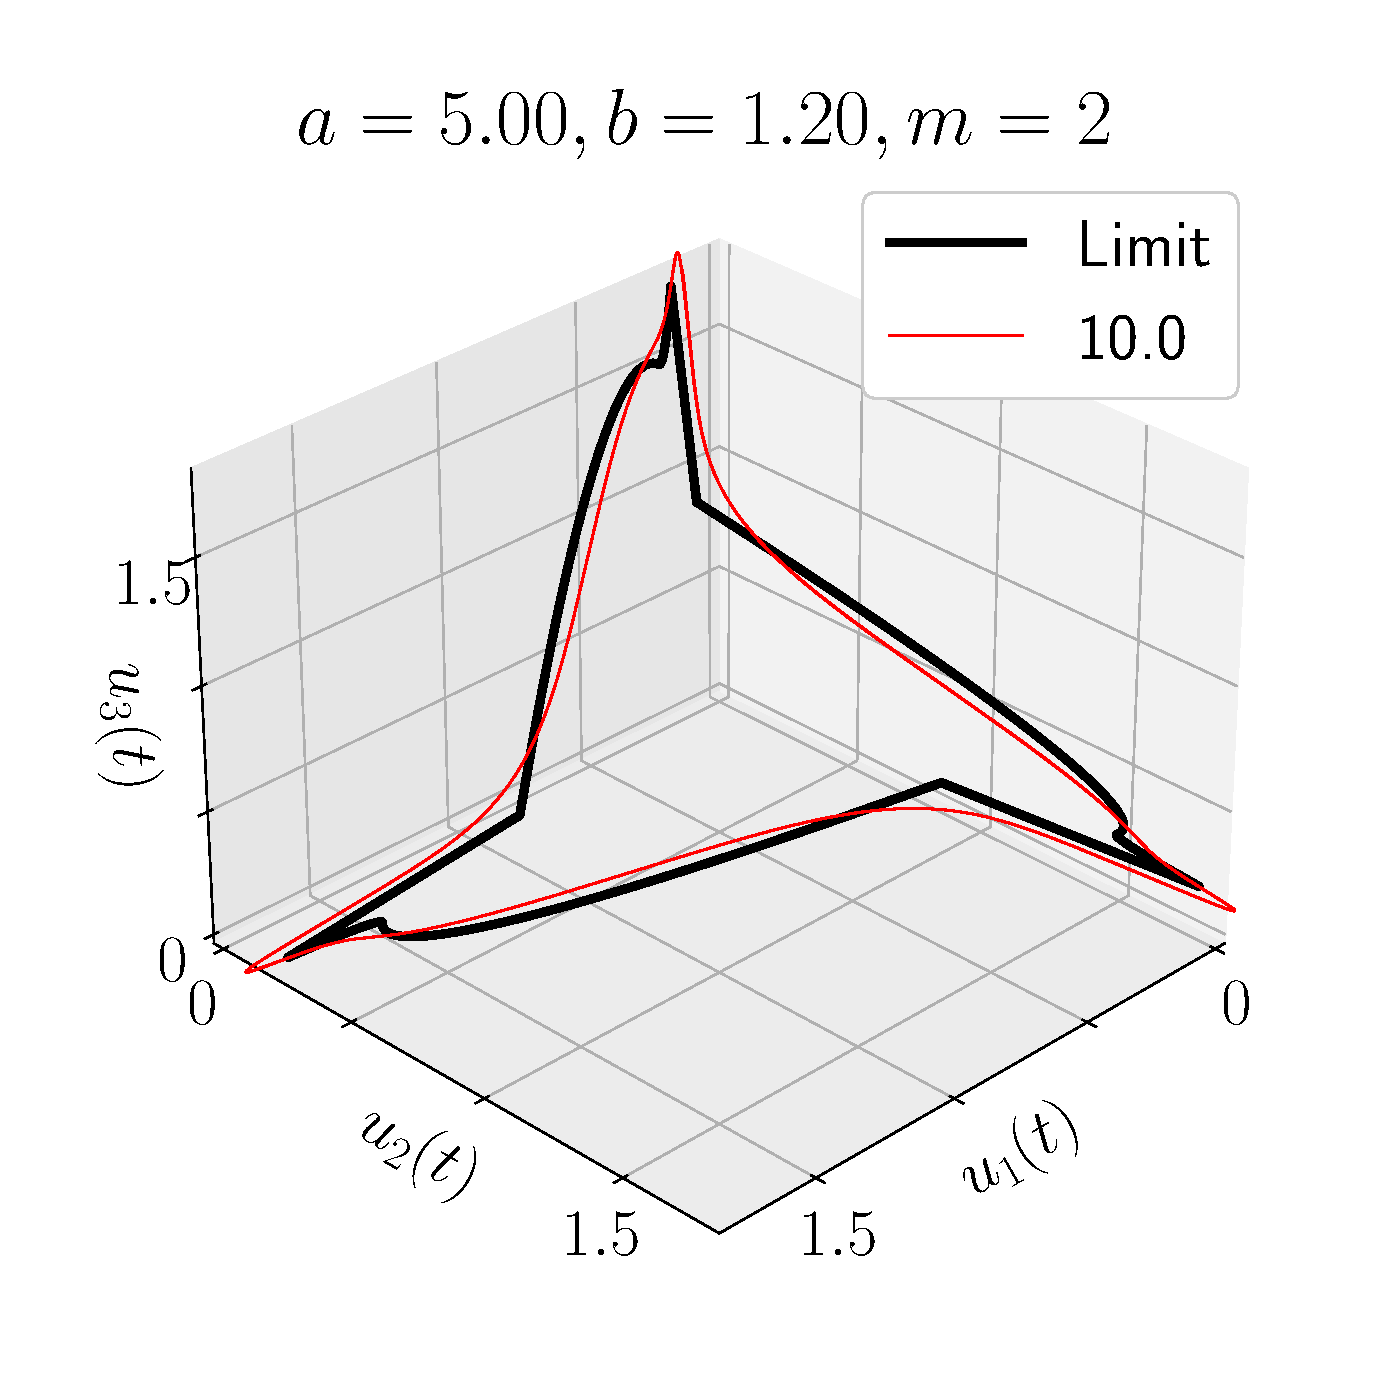
\includegraphics[width=0.48\textwidth]{alpha_5_beta_1p2_3d_10.eps}\hfill
	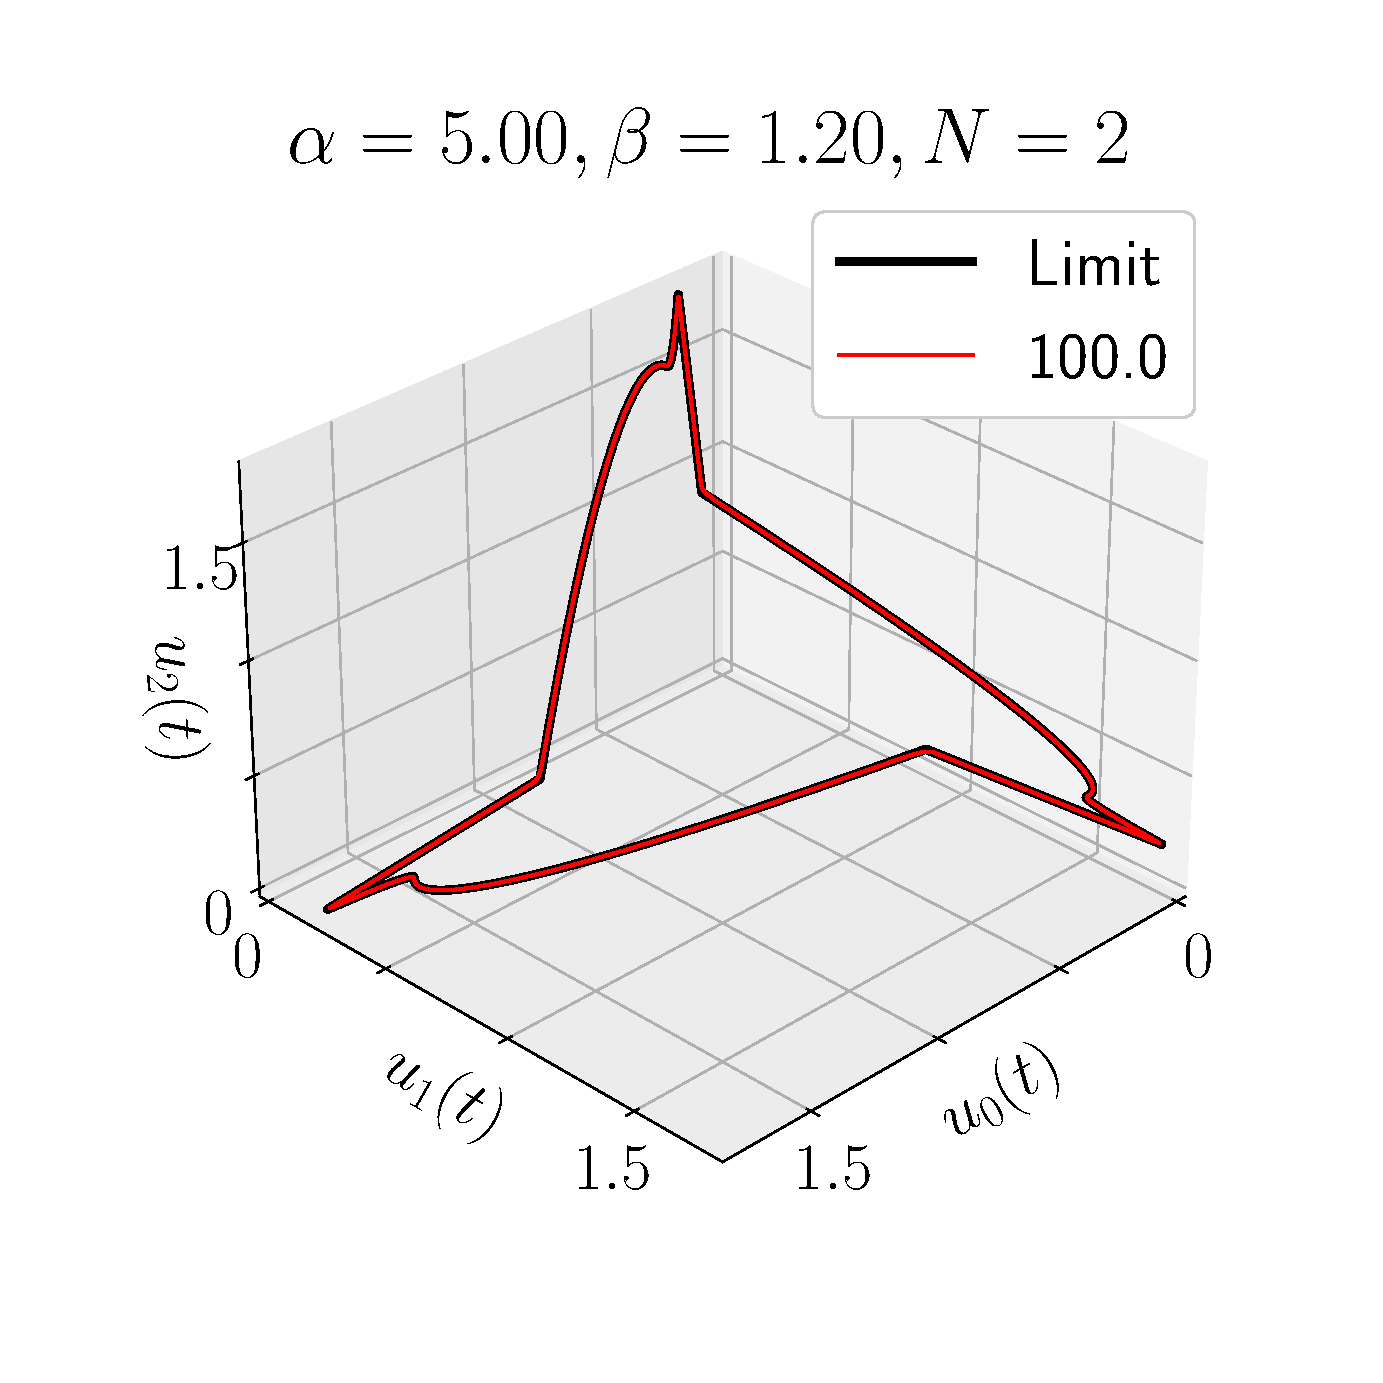
\includegraphics[width=0.48\textwidth]{alpha_5_beta_1p2_3d_100.eps}
	\caption{Иллюстрация периодического решения предельной системы \eqref{eq:system_relay} в псевдофазовом пространстве в сравнении с решением системы \eqref{eq:mg_full_renormed} при $\gamma = 10$ (слева) и $\gamma = 100$ (справа).}
	\label{fig:solution_3d}
\end{figure}

%TODO: взять статью из диффуров и скопировать оттуда ещё картинки

\section{Выводы к главе 2}\label{sec:ch2/sect5}

В данной главе проведено исследование предельного при $\gamma \to +\infty$ объекта для системы \eqref{eq:mg_full_renormed}, описывающей полносвязную систему генераторов Мэки--Гласса. Для релейной системы \eqref{eq:system_relay} показано (при некоторых ограничениях на параметры) существование периодического режима в виде <<дискретной бегущей волны>> --- режима, при котором компоненты решения отличаются друг от друга сдвигом (в некотором порядке) на фиксированную величину. Явное описание решения и ограничений на параметры дано в теореме \ref{thm:mg_auxiliary_main}. В теореме \ref{thm:relay_main} приведено семейство параметров с более простым аналитическим описанием.

% Картинки: см. ноутбуки 2022-04-30-численный-счёт, 2024-01-27-картинки-в-диссер
